% Options for packages loaded elsewhere
\PassOptionsToPackage{unicode}{hyperref}
\PassOptionsToPackage{hyphens}{url}
\PassOptionsToPackage{dvipsnames,svgnames,x11names}{xcolor}
%
\documentclass[
  letterpaper,
  DIV=11,
  numbers=noendperiod]{scrreport}

\usepackage{amsmath,amssymb}
\usepackage{iftex}
\ifPDFTeX
  \usepackage[T1]{fontenc}
  \usepackage[utf8]{inputenc}
  \usepackage{textcomp} % provide euro and other symbols
\else % if luatex or xetex
  \usepackage{unicode-math}
  \defaultfontfeatures{Scale=MatchLowercase}
  \defaultfontfeatures[\rmfamily]{Ligatures=TeX,Scale=1}
\fi
\usepackage{lmodern}
\ifPDFTeX\else  
    % xetex/luatex font selection
\fi
% Use upquote if available, for straight quotes in verbatim environments
\IfFileExists{upquote.sty}{\usepackage{upquote}}{}
\IfFileExists{microtype.sty}{% use microtype if available
  \usepackage[]{microtype}
  \UseMicrotypeSet[protrusion]{basicmath} % disable protrusion for tt fonts
}{}
\makeatletter
\@ifundefined{KOMAClassName}{% if non-KOMA class
  \IfFileExists{parskip.sty}{%
    \usepackage{parskip}
  }{% else
    \setlength{\parindent}{0pt}
    \setlength{\parskip}{6pt plus 2pt minus 1pt}}
}{% if KOMA class
  \KOMAoptions{parskip=half}}
\makeatother
\usepackage{xcolor}
\setlength{\emergencystretch}{3em} % prevent overfull lines
\setcounter{secnumdepth}{5}
% Make \paragraph and \subparagraph free-standing
\ifx\paragraph\undefined\else
  \let\oldparagraph\paragraph
  \renewcommand{\paragraph}[1]{\oldparagraph{#1}\mbox{}}
\fi
\ifx\subparagraph\undefined\else
  \let\oldsubparagraph\subparagraph
  \renewcommand{\subparagraph}[1]{\oldsubparagraph{#1}\mbox{}}
\fi

\usepackage{color}
\usepackage{fancyvrb}
\newcommand{\VerbBar}{|}
\newcommand{\VERB}{\Verb[commandchars=\\\{\}]}
\DefineVerbatimEnvironment{Highlighting}{Verbatim}{commandchars=\\\{\}}
% Add ',fontsize=\small' for more characters per line
\usepackage{framed}
\definecolor{shadecolor}{RGB}{241,243,245}
\newenvironment{Shaded}{\begin{snugshade}}{\end{snugshade}}
\newcommand{\AlertTok}[1]{\textcolor[rgb]{0.68,0.00,0.00}{#1}}
\newcommand{\AnnotationTok}[1]{\textcolor[rgb]{0.37,0.37,0.37}{#1}}
\newcommand{\AttributeTok}[1]{\textcolor[rgb]{0.40,0.45,0.13}{#1}}
\newcommand{\BaseNTok}[1]{\textcolor[rgb]{0.68,0.00,0.00}{#1}}
\newcommand{\BuiltInTok}[1]{\textcolor[rgb]{0.00,0.23,0.31}{#1}}
\newcommand{\CharTok}[1]{\textcolor[rgb]{0.13,0.47,0.30}{#1}}
\newcommand{\CommentTok}[1]{\textcolor[rgb]{0.37,0.37,0.37}{#1}}
\newcommand{\CommentVarTok}[1]{\textcolor[rgb]{0.37,0.37,0.37}{\textit{#1}}}
\newcommand{\ConstantTok}[1]{\textcolor[rgb]{0.56,0.35,0.01}{#1}}
\newcommand{\ControlFlowTok}[1]{\textcolor[rgb]{0.00,0.23,0.31}{#1}}
\newcommand{\DataTypeTok}[1]{\textcolor[rgb]{0.68,0.00,0.00}{#1}}
\newcommand{\DecValTok}[1]{\textcolor[rgb]{0.68,0.00,0.00}{#1}}
\newcommand{\DocumentationTok}[1]{\textcolor[rgb]{0.37,0.37,0.37}{\textit{#1}}}
\newcommand{\ErrorTok}[1]{\textcolor[rgb]{0.68,0.00,0.00}{#1}}
\newcommand{\ExtensionTok}[1]{\textcolor[rgb]{0.00,0.23,0.31}{#1}}
\newcommand{\FloatTok}[1]{\textcolor[rgb]{0.68,0.00,0.00}{#1}}
\newcommand{\FunctionTok}[1]{\textcolor[rgb]{0.28,0.35,0.67}{#1}}
\newcommand{\ImportTok}[1]{\textcolor[rgb]{0.00,0.46,0.62}{#1}}
\newcommand{\InformationTok}[1]{\textcolor[rgb]{0.37,0.37,0.37}{#1}}
\newcommand{\KeywordTok}[1]{\textcolor[rgb]{0.00,0.23,0.31}{#1}}
\newcommand{\NormalTok}[1]{\textcolor[rgb]{0.00,0.23,0.31}{#1}}
\newcommand{\OperatorTok}[1]{\textcolor[rgb]{0.37,0.37,0.37}{#1}}
\newcommand{\OtherTok}[1]{\textcolor[rgb]{0.00,0.23,0.31}{#1}}
\newcommand{\PreprocessorTok}[1]{\textcolor[rgb]{0.68,0.00,0.00}{#1}}
\newcommand{\RegionMarkerTok}[1]{\textcolor[rgb]{0.00,0.23,0.31}{#1}}
\newcommand{\SpecialCharTok}[1]{\textcolor[rgb]{0.37,0.37,0.37}{#1}}
\newcommand{\SpecialStringTok}[1]{\textcolor[rgb]{0.13,0.47,0.30}{#1}}
\newcommand{\StringTok}[1]{\textcolor[rgb]{0.13,0.47,0.30}{#1}}
\newcommand{\VariableTok}[1]{\textcolor[rgb]{0.07,0.07,0.07}{#1}}
\newcommand{\VerbatimStringTok}[1]{\textcolor[rgb]{0.13,0.47,0.30}{#1}}
\newcommand{\WarningTok}[1]{\textcolor[rgb]{0.37,0.37,0.37}{\textit{#1}}}

\providecommand{\tightlist}{%
  \setlength{\itemsep}{0pt}\setlength{\parskip}{0pt}}\usepackage{longtable,booktabs,array}
\usepackage{calc} % for calculating minipage widths
% Correct order of tables after \paragraph or \subparagraph
\usepackage{etoolbox}
\makeatletter
\patchcmd\longtable{\par}{\if@noskipsec\mbox{}\fi\par}{}{}
\makeatother
% Allow footnotes in longtable head/foot
\IfFileExists{footnotehyper.sty}{\usepackage{footnotehyper}}{\usepackage{footnote}}
\makesavenoteenv{longtable}
\usepackage{graphicx}
\makeatletter
\def\maxwidth{\ifdim\Gin@nat@width>\linewidth\linewidth\else\Gin@nat@width\fi}
\def\maxheight{\ifdim\Gin@nat@height>\textheight\textheight\else\Gin@nat@height\fi}
\makeatother
% Scale images if necessary, so that they will not overflow the page
% margins by default, and it is still possible to overwrite the defaults
% using explicit options in \includegraphics[width, height, ...]{}
\setkeys{Gin}{width=\maxwidth,height=\maxheight,keepaspectratio}
% Set default figure placement to htbp
\makeatletter
\def\fps@figure{htbp}
\makeatother

\KOMAoption{captions}{tableheading}
\makeatletter
\makeatother
\makeatletter
\@ifpackageloaded{bookmark}{}{\usepackage{bookmark}}
\makeatother
\makeatletter
\@ifpackageloaded{caption}{}{\usepackage{caption}}
\AtBeginDocument{%
\ifdefined\contentsname
  \renewcommand*\contentsname{Table of contents}
\else
  \newcommand\contentsname{Table of contents}
\fi
\ifdefined\listfigurename
  \renewcommand*\listfigurename{List of Figures}
\else
  \newcommand\listfigurename{List of Figures}
\fi
\ifdefined\listtablename
  \renewcommand*\listtablename{List of Tables}
\else
  \newcommand\listtablename{List of Tables}
\fi
\ifdefined\figurename
  \renewcommand*\figurename{Figure}
\else
  \newcommand\figurename{Figure}
\fi
\ifdefined\tablename
  \renewcommand*\tablename{Table}
\else
  \newcommand\tablename{Table}
\fi
}
\@ifpackageloaded{float}{}{\usepackage{float}}
\floatstyle{ruled}
\@ifundefined{c@chapter}{\newfloat{codelisting}{h}{lop}}{\newfloat{codelisting}{h}{lop}[chapter]}
\floatname{codelisting}{Listing}
\newcommand*\listoflistings{\listof{codelisting}{List of Listings}}
\makeatother
\makeatletter
\@ifpackageloaded{caption}{}{\usepackage{caption}}
\@ifpackageloaded{subcaption}{}{\usepackage{subcaption}}
\makeatother
\makeatletter
\@ifpackageloaded{tcolorbox}{}{\usepackage[skins,breakable]{tcolorbox}}
\makeatother
\makeatletter
\@ifundefined{shadecolor}{\definecolor{shadecolor}{rgb}{.97, .97, .97}}
\makeatother
\makeatletter
\makeatother
\makeatletter
\makeatother
\ifLuaTeX
  \usepackage{selnolig}  % disable illegal ligatures
\fi
\IfFileExists{bookmark.sty}{\usepackage{bookmark}}{\usepackage{hyperref}}
\IfFileExists{xurl.sty}{\usepackage{xurl}}{} % add URL line breaks if available
\urlstyle{same} % disable monospaced font for URLs
\hypersetup{
  pdftitle={Efficacy of fungicides against brown spot of pear in Argentina},
  pdfauthor={Tudela et al.},
  colorlinks=true,
  linkcolor={blue},
  filecolor={Maroon},
  citecolor={Blue},
  urlcolor={Blue},
  pdfcreator={LaTeX via pandoc}}

\title{Efficacy of fungicides against brown spot of pear in Argentina}
\author{Tudela et al.}
\date{}

\begin{document}
\maketitle
\ifdefined\Shaded\renewenvironment{Shaded}{\begin{tcolorbox}[interior hidden, borderline west={3pt}{0pt}{shadecolor}, enhanced, frame hidden, sharp corners, boxrule=0pt, breakable]}{\end{tcolorbox}}\fi

\renewcommand*\contentsname{Table of contents}
{
\hypersetup{linkcolor=}
\setcounter{tocdepth}{2}
\tableofcontents
}
\bookmarksetup{startatroot}

\hypertarget{abstract}{%
\chapter*{Abstract}\label{abstract}}
\addcontentsline{toc}{chapter}{Abstract}

\markboth{Abstract}{Abstract}

Authors: Marisa Andrea Aluminé Tudela*, María Cecilia Lutz, Gustavo
Nestor Giménez, Susana Noemí Di Masi, Graciela Noemí Pose, Dolores Del
Brío, Juan Pablo Edwards Molina

*Corresponding autor (tudela.alumine@inta.gob.ar)
ORCID:0000-0001-8298-8064

Brown spot of pear (BSP), a fungal disease of importance in Europe, has
been recently detected for the first time in pear orchards in the Alto
Valle of Río Negro (Patagonia), Argentina, South America. The disease is
caused by \emph{Stemphylium vesicarium} and its main symptoms are
lesions in fruits and leaves. To assess counteracting measures against
BSP, the effects of four fungicides were tested to evaluate \emph{in
vitro} efficacy against mycelial growth and spore germination of native
\emph{S. vesicarium} strains, and preventive and curative control of
lesion development in pear fruit `D'Anjou' var. In addition, the
activities of two selected fungicides were determined through in-field
assays. The fungicides tested were chosen according to their commercial
availability and registration in pear crops and included: pyraclostrobin
+ boscalid (Bellis®); ziram (Ziram®); captan (Merpan®); and
\emph{Melaleuca alternifolia} extract (Timorex®). Bellis® presented the
lowest EC50 values in germination and mycelial growth tests. Ziram® and
Merpan® were also very effective in inhibiting germination. The
plant-based biofungicide Timorex® did not achieve satisfactory
effectiveness in in vitro trials, nor in bioassays after preventive and
curative treatments. Bioassay results showed that preventive measures
using Bellis®, Ziram®, or Merpan® were effective in reducing disease
severity and suggested that BSP could be controlled by adequate
selection of treatment time.

\begin{figure}

{\centering 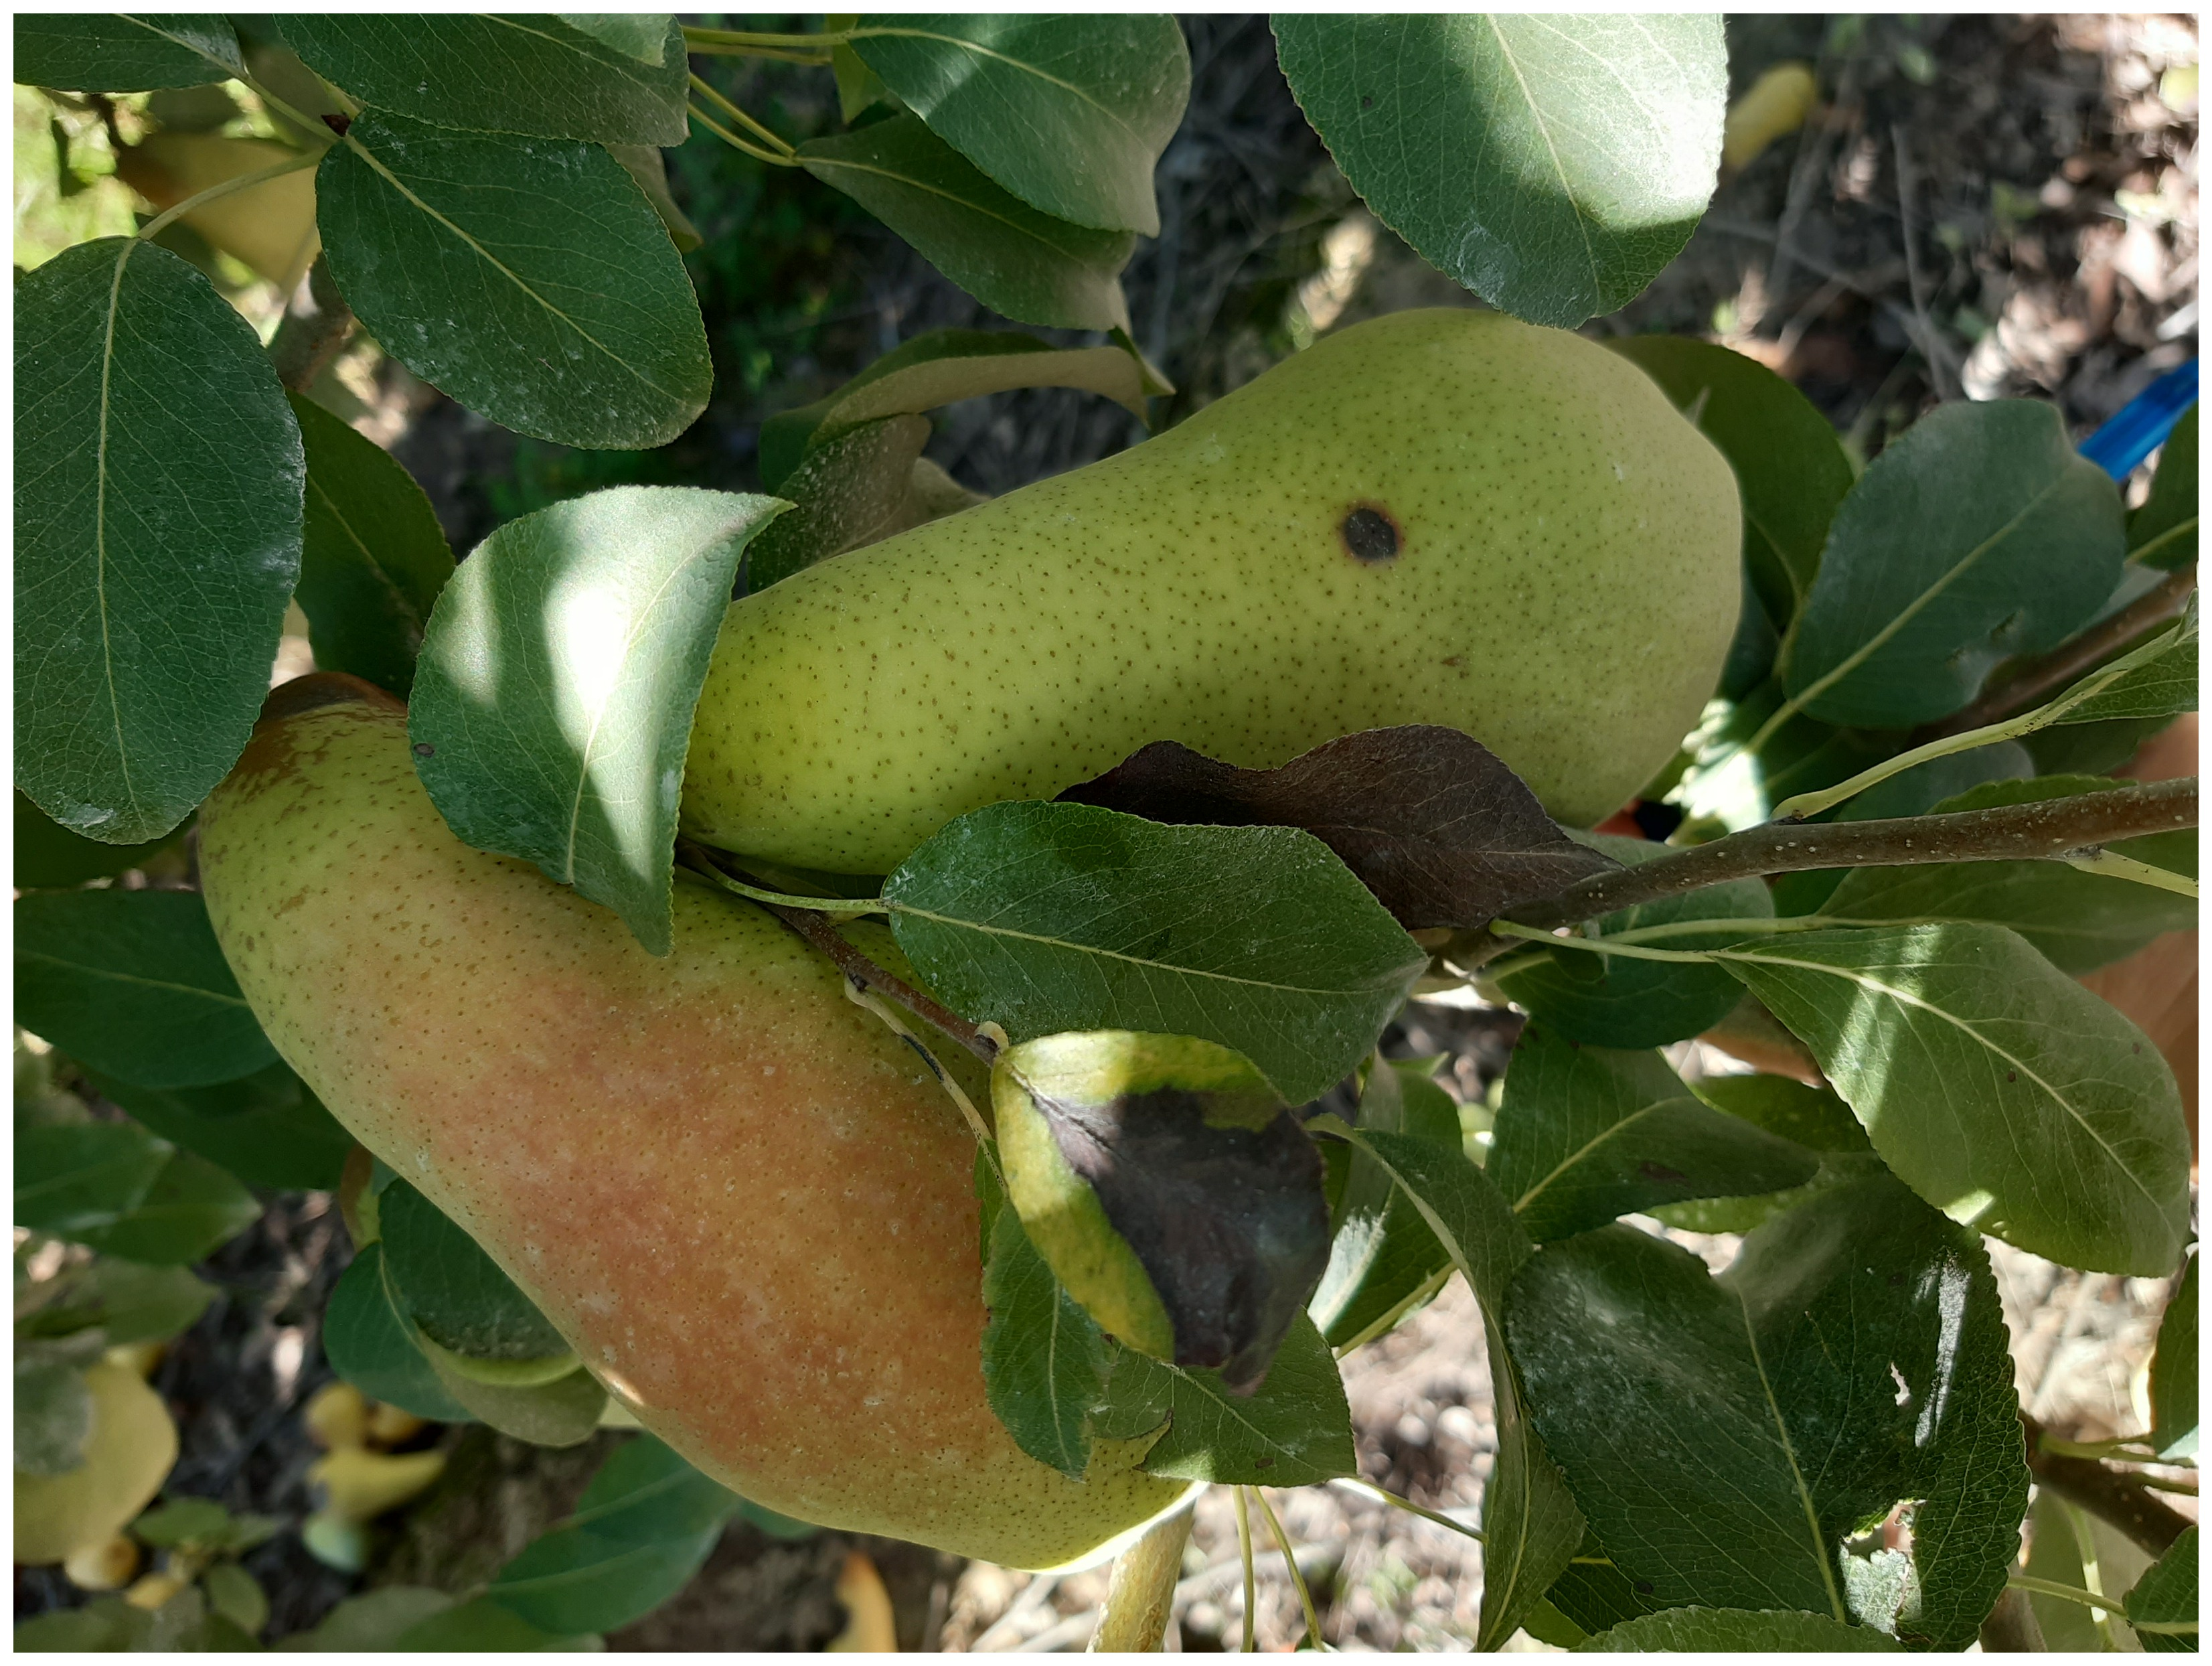
\includegraphics[width=0.5\textwidth,height=\textheight]{images/abate_border.png}

}

\caption{Abate pear cultivar with symptoms of brown spot caused by
\emph{Stemphylium vesicarium}}

\end{figure}

\begin{figure}

{\centering 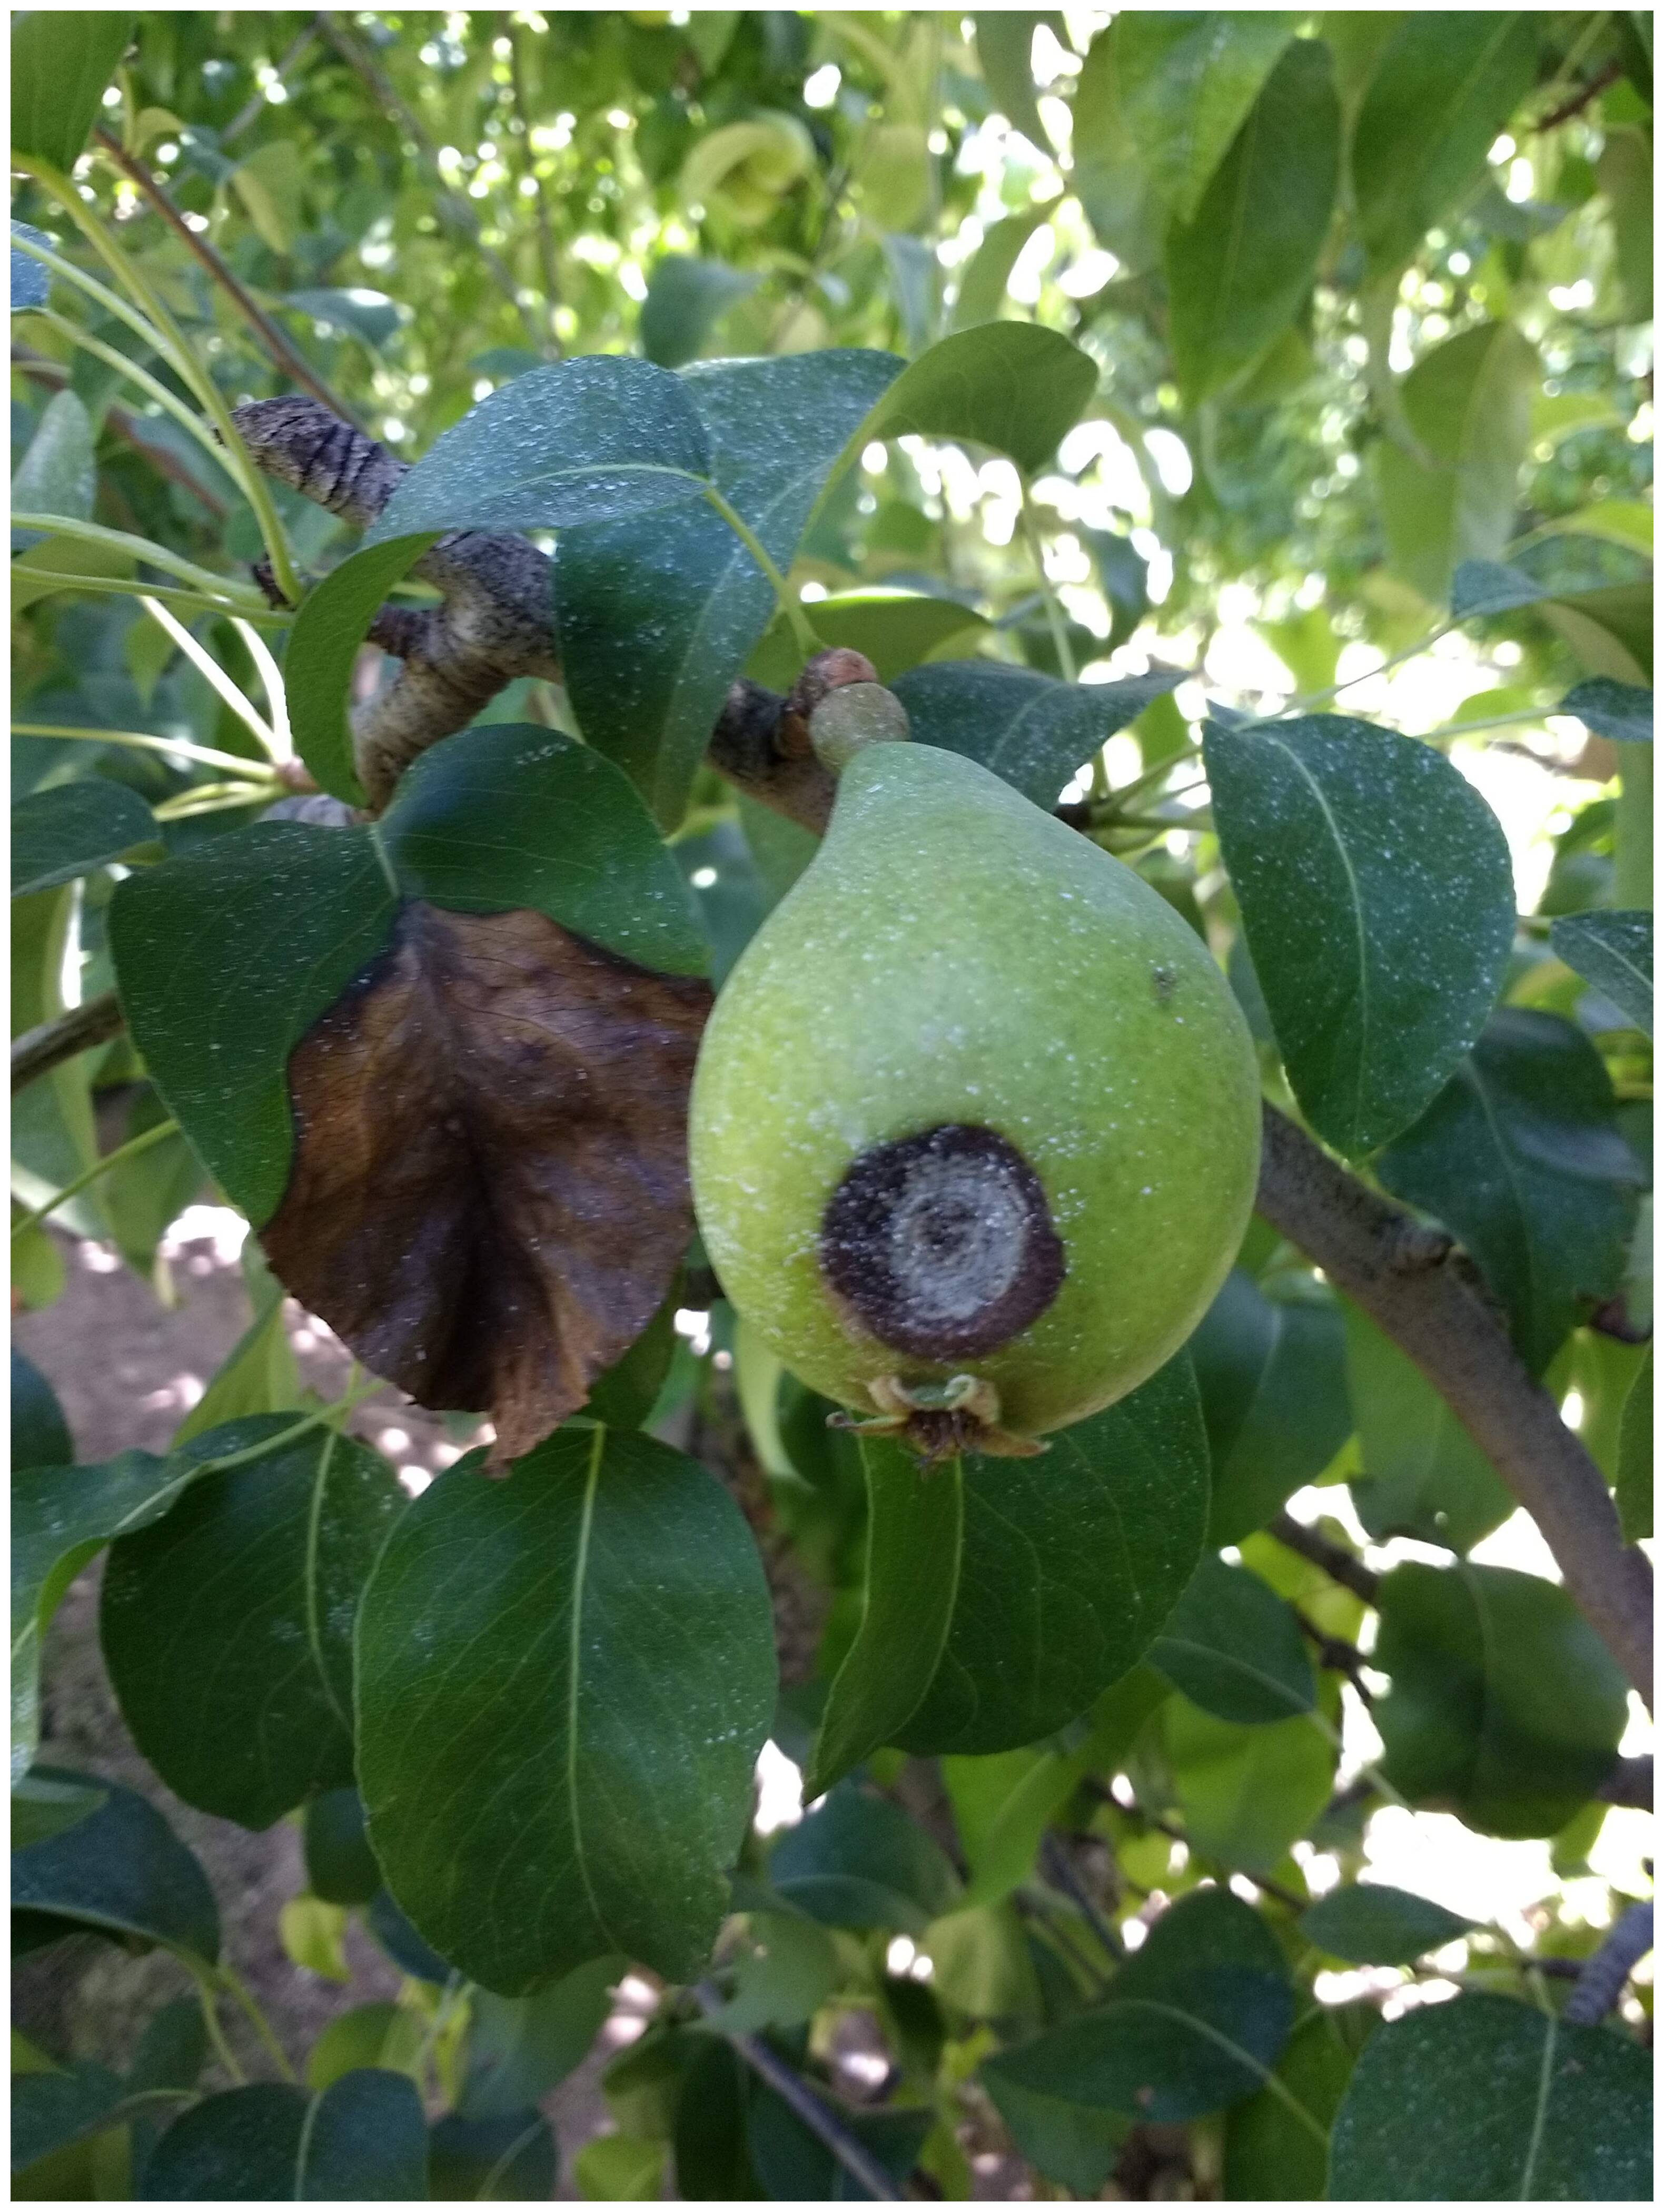
\includegraphics[width=0.5\textwidth,height=\textheight]{images/danjou_border.png}

}

\caption{Danjou pear cultivar with symptoms of brown spot caused by
\emph{Stemphylium vesicarium}}

\end{figure}

\bookmarksetup{startatroot}

\hypertarget{in-vitro-experiments}{%
\chapter{In vitro experiments}\label{in-vitro-experiments}}

\hypertarget{mycelial-growth}{%
\section{Mycelial growth}\label{mycelial-growth}}

\begin{Shaded}
\begin{Highlighting}[]
\NormalTok{raw }\OtherTok{\textless{}{-}} \FunctionTok{import}\NormalTok{(}\StringTok{"data/mycelial\_growth.csv"}\NormalTok{, }\AttributeTok{dec=}\StringTok{","}\NormalTok{)}

\NormalTok{dat }\OtherTok{\textless{}{-}}\NormalTok{ raw }\SpecialCharTok{\%\textgreater{}\%} 
  \FunctionTok{mutate\_at}\NormalTok{(}\FunctionTok{vars}\NormalTok{(dose, colony\_diameter), as.numeric) }\SpecialCharTok{\%\textgreater{}\%} 
  \FunctionTok{mutate\_at}\NormalTok{(}\FunctionTok{vars}\NormalTok{(fungicide, strain, experiment, plate), as.factor) }\SpecialCharTok{\%\textgreater{}\%} 
  \FunctionTok{mutate}\NormalTok{(}\AttributeTok{curve\_id =} \FunctionTok{interaction}\NormalTok{(fungicide}\SpecialCharTok{:}\NormalTok{strain}\SpecialCharTok{:}\NormalTok{experiment)) }
\end{Highlighting}
\end{Shaded}

Data structure

\begin{Shaded}
\begin{Highlighting}[]
\FunctionTok{ftable}\NormalTok{(}\FunctionTok{xtabs}\NormalTok{(}\SpecialCharTok{\textasciitilde{}}\NormalTok{ fungicide }\SpecialCharTok{+}\NormalTok{ strain }\SpecialCharTok{+}\NormalTok{ experiment }\SpecialCharTok{+}\NormalTok{ dose, dat))}
\end{Highlighting}
\end{Shaded}

\begin{verbatim}
                            dose 0 0.01 0.1 0.5 1 10 50 100 500 1000
fungicide strain experiment                                         
Bellis    S20    1               3    3   3   0 3  3  3   3   0    0
                 2               3    3   3   0 3  3  3   3   0    0
                 3               3    3   3   0 3  3  3   3   0    0
          S23    1               3    3   3   0 3  3  3   3   0    0
                 2               3    3   3   0 3  3  3   3   0    0
                 3               3    3   3   0 3  3  3   3   0    0
          S8     1               3    3   3   0 3  3  3   3   0    0
                 2               3    3   3   0 3  3  3   3   0    0
                 3               3    3   3   0 3  3  3   3   0    0
Merpan    S20    1               3    0   3   0 3  3  0   3   3    3
                 2               3    0   3   0 3  3  0   3   3    3
                 3               3    0   3   0 3  3  0   3   3    3
          S23    1               3    0   3   0 3  3  0   3   3    3
                 2               3    0   3   0 3  3  0   3   3    3
                 3               3    0   3   0 3  3  0   3   3    3
          S8     1               3    0   3   0 3  3  0   3   3    3
                 2               3    0   3   0 3  3  0   3   3    3
                 3               3    0   3   0 3  3  0   3   3    3
Timorex   S20    1               3    0   3   0 3  3  0   3   3    3
                 2               3    0   3   0 3  3  0   3   3    3
                 3               3    0   3   0 3  3  0   3   3    3
          S23    1               3    0   3   0 3  3  0   3   3    3
                 2               3    0   3   0 3  3  0   3   3    3
                 3               3    0   3   0 3  3  0   3   3    3
          S8     1               3    0   3   0 3  3  0   3   3    3
                 2               3    0   3   0 3  3  0   3   3    3
                 3               3    0   3   0 3  3  0   3   3    3
Ziram     S20    1               3    0   3   3 3  3  3   3   0    0
                 2               3    0   3   3 3  3  3   3   0    0
                 3               3    0   3   3 3  3  3   3   0    0
          S23    1               3    0   3   3 3  3  3   3   0    0
                 2               3    0   3   3 3  3  3   3   0    0
                 3               3    0   3   3 3  3  3   3   0    0
          S8     1               3    0   3   3 3  3  3   3   0    0
                 2               3    0   3   3 3  3  3   3   0    0
                 3               3    0   3   3 3  3  3   3   0    0
\end{verbatim}

\begin{Shaded}
\begin{Highlighting}[]
\FunctionTok{str}\NormalTok{(dat)}
\end{Highlighting}
\end{Shaded}

\begin{verbatim}
'data.frame':   756 obs. of  7 variables:
 $ fungicide      : Factor w/ 4 levels "Bellis","Merpan",..: 1 1 1 1 1 1 1 1 1 1 ...
 $ strain         : Factor w/ 3 levels "S20","S23","S8": 2 2 2 1 1 1 3 3 3 2 ...
 $ experiment     : Factor w/ 3 levels "1","2","3": 1 1 1 1 1 1 1 1 1 1 ...
 $ dose           : num  0 0 0 0 0 0 0 0 0 100 ...
 $ plate          : Factor w/ 3 levels "1","2","3": 1 2 3 1 2 3 1 2 3 1 ...
 $ colony_diameter: num  53 55 56 52 53 52 51 51 52 0 ...
 $ curve_id       : Factor w/ 36 levels "Bellis:S20:1",..: 4 4 4 1 1 1 7 7 7 4 ...
\end{verbatim}

Dose-response curves fitting by meta-analysis approach

\begin{Shaded}
\begin{Highlighting}[]
\CommentTok{\# verify drc\_per\_strain.R}
\NormalTok{mod\_mg }\OtherTok{\textless{}{-}} \FunctionTok{metadrm}\NormalTok{(colony\_diameter }\SpecialCharTok{\textasciitilde{}}\NormalTok{ dose, }
               \AttributeTok{data=}\NormalTok{dat,}
               \AttributeTok{fct=}\FunctionTok{LL.3}\NormalTok{(),}
               \AttributeTok{ind=}\NormalTok{curve\_id,}
               \AttributeTok{cid2=}\NormalTok{fungicide,}
               \AttributeTok{struct=}\StringTok{"UN"}\NormalTok{)}
\FunctionTok{save}\NormalTok{(mod\_mg, }\AttributeTok{file=} \StringTok{"models/invitro\_mg.rds"}\NormalTok{)}
\end{Highlighting}
\end{Shaded}

\begin{Shaded}
\begin{Highlighting}[]
\FunctionTok{load}\NormalTok{(}\StringTok{"models/invitro\_mg.rds"}\NormalTok{)}
\FunctionTok{summary}\NormalTok{(mod\_mg)}
\end{Highlighting}
\end{Shaded}

\begin{verbatim}

Two-stage meta-analysis dose-response model
Model fitted: Log-logistic (ED50 as parameter) with lower limit at 0

Call:
metadrm(formula = colony_diameter ~ dose, fct = LL.3(), ind = curve_id, 
    data = dat, cid2 = fungicide, struct = "UN")

Variance estimates:
            estim    sqrt
tau^2.1    0.0023  0.0481
tau^2.2    8.1930  2.8623
tau^2.3    0.0001  0.0076

               rho.b:(I  rho.d:(I  rho.e:(I
b:(Intercept)         1   -0.0949    0.9136
d:(Intercept)   -0.0949         1   -0.4915
e:(Intercept)    0.9136   -0.4915         1


Coefficients:
             Estimate     Std.Err t value              Pr(>|t|)    
b:Bellis    0.5795367   0.0182490 31.7572 < 0.00000000000000022 ***
b:Merpan    0.3611793   0.0183369 19.6968 < 0.00000000000000022 ***
b:Timorex   0.3490411   0.0324495 10.7565 < 0.00000000000000022 ***
b:Ziram     0.3926960   0.0202379 19.4040 < 0.00000000000000022 ***
d:Bellis   51.3746461   0.9890286 51.9446 < 0.00000000000000022 ***
d:Merpan   52.5139150   1.0667613 49.2274 < 0.00000000000000022 ***
d:Timorex  49.9869522   1.3972223 35.7759 < 0.00000000000000022 ***
d:Ziram    53.0642566   1.1218557 47.3004 < 0.00000000000000022 ***
e:Bellis    0.0297542   0.0027299 10.8994 < 0.00000000000000022 ***
e:Merpan   24.5154698   1.6200305 15.1327 < 0.00000000000000022 ***
e:Timorex 112.8372474  22.1680049  5.0901           0.000001779 ***
e:Ziram     6.4555590   0.6162007 10.4764 < 0.00000000000000022 ***
---
Signif. codes:  0 '***' 0.001 '**' 0.01 '*' 0.05 '.' 0.1 ' ' 1
\end{verbatim}

EC50 Estimates

\begin{Shaded}
\begin{Highlighting}[]
\NormalTok{ec50s }\OtherTok{\textless{}{-}} \FunctionTok{ED}\NormalTok{(mod\_mg, }\AttributeTok{respLev=}\FunctionTok{c}\NormalTok{(}\DecValTok{50}\NormalTok{)) }\SpecialCharTok{\%\textgreater{}\%}\NormalTok{ data.frame}
\end{Highlighting}
\end{Shaded}

\begin{verbatim}

Estimated effective doses

                Estimate  Std. Error
e:Bellis:50    0.0297542   0.0027299
e:Merpan:50   24.5154698   1.6200305
e:Timorex:50 112.8372474  22.1680049
e:Ziram:50     6.4555590   0.6162007
\end{verbatim}

\begin{Shaded}
\begin{Highlighting}[]
\CommentTok{\# coef\_mod\_mg \textless{}{-} summary(mod\_mg) \%\textgreater{}\% data.frame \%\textgreater{}\% }
\CommentTok{\#   rownames\_to\_column("param")  \%\textgreater{}\% }
\CommentTok{\#   separate(param, c("param", "fungicide"))}
\CommentTok{\# ec50s \textless{}{-} coef\_mod\_mg \%\textgreater{}\% filter(param=="e") }
\CommentTok{\# ec50s}
\end{Highlighting}
\end{Shaded}

Comparing fungicides EC50

As we compare EC50 ratios between fungicides, if the confidence interval
does not contain 1, fungicides differ among them:

\begin{Shaded}
\begin{Highlighting}[]
\NormalTok{ed\_comp }\OtherTok{\textless{}{-}} \FunctionTok{EDcomp}\NormalTok{(mod\_mg, }
                  \AttributeTok{percVec=}\FunctionTok{c}\NormalTok{(}\DecValTok{50}\NormalTok{), }
                  \AttributeTok{percMat=}\FunctionTok{rbind}\NormalTok{(}\FunctionTok{c}\NormalTok{(}\DecValTok{1}\NormalTok{,}\DecValTok{1}\NormalTok{,}\DecValTok{1}\NormalTok{,}\DecValTok{1}\NormalTok{)), }
                  \AttributeTok{interval=}\StringTok{"fieller"}\NormalTok{) }\SpecialCharTok{\%\textgreater{}\%} 
\NormalTok{      data.frame }\SpecialCharTok{\%\textgreater{}\%} 
  \FunctionTok{rownames\_to\_column}\NormalTok{(}\StringTok{"comp"}\NormalTok{) }\SpecialCharTok{\%\textgreater{}\%}
  \FunctionTok{rowwise}\NormalTok{() }\SpecialCharTok{\%\textgreater{}\%} 
  \FunctionTok{mutate}\NormalTok{(}\AttributeTok{relative\_to\_one =} \FunctionTok{f}\NormalTok{(Lower, Upper, }\DecValTok{1}\NormalTok{)) }\CommentTok{\# \%\textgreater{}\% }
\end{Highlighting}
\end{Shaded}

\begin{verbatim}

Estimated ratios of effect doses

                        Estimate       Lower       Upper
Bellis/Merpan:50/50   0.00121369  0.00095935  0.00151054
Bellis/Timorex:50/50  0.00026369  0.00017897  0.00044300
Bellis/Ziram:50/50    0.00460909  0.00353519  0.00602624
Merpan/Timorex:50/50  0.21726398  0.15162515  0.36083619
Merpan/Ziram:50/50    3.79757505  3.03655193  4.84141476
Timorex/Ziram:50/50  17.47908235 10.38447082 25.87541262
\end{verbatim}

\begin{Shaded}
\begin{Highlighting}[]
  \CommentTok{\# as\_huxtable() \%\textgreater{}\% }
  \CommentTok{\# set\_number\_format(1)}
\NormalTok{ed\_comp}
\end{Highlighting}
\end{Shaded}

\begin{verbatim}
# A tibble: 6 x 5
# Rowwise: 
  comp                  Estimate     Lower     Upper relative_to_one
  <chr>                    <dbl>     <dbl>     <dbl> <chr>          
1 Bellis/Merpan:50/50   0.00121   0.000959  0.00151  below          
2 Bellis/Timorex:50/50  0.000264  0.000179  0.000443 below          
3 Bellis/Ziram:50/50    0.00461   0.00354   0.00603  below          
4 Merpan/Timorex:50/50  0.217     0.152     0.361    below          
5 Merpan/Ziram:50/50    3.80      3.04      4.84     above          
6 Timorex/Ziram:50/50  17.5      10.4      25.9      above          
\end{verbatim}

\begin{Shaded}
\begin{Highlighting}[]
\NormalTok{ed\_comp }\SpecialCharTok{\%\textgreater{}\%} 
  \FunctionTok{ggplot}\NormalTok{()}\SpecialCharTok{+} 
  \FunctionTok{aes}\NormalTok{(}\AttributeTok{x=}\NormalTok{comp, }\AttributeTok{y=}\NormalTok{Estimate) }\SpecialCharTok{+} 
  \FunctionTok{geom\_pointrange}\NormalTok{(}\FunctionTok{aes}\NormalTok{(}\AttributeTok{ymin =}\NormalTok{ Lower, }\AttributeTok{ymax =}\NormalTok{ Upper, }\AttributeTok{col=}\NormalTok{relative\_to\_one))}\SpecialCharTok{+}     
  \FunctionTok{geom\_hline}\NormalTok{(}\AttributeTok{yintercept =} \DecValTok{1}\NormalTok{, }\AttributeTok{linetype=}\DecValTok{2}\NormalTok{)}\SpecialCharTok{+}
  \CommentTok{\# scale\_y\_log10()+}
  \FunctionTok{coord\_flip}\NormalTok{() }\SpecialCharTok{+} 
  \FunctionTok{labs}\NormalTok{(}\AttributeTok{col=}\StringTok{"Relative to 1"}\NormalTok{)}
\end{Highlighting}
\end{Shaded}

\begin{Shaded}
\begin{Highlighting}[]
\NormalTok{dat }\SpecialCharTok{\%\textgreater{}\%} 
  \FunctionTok{ggplot}\NormalTok{()}\SpecialCharTok{+}
  \FunctionTok{aes}\NormalTok{(}\AttributeTok{x=}\NormalTok{dose}\FloatTok{+0.0001}\NormalTok{, }\AttributeTok{y=}\NormalTok{colony\_diameter, }\AttributeTok{col=}\NormalTok{fungicide) }\SpecialCharTok{+}
  \FunctionTok{geom\_point}\NormalTok{(}\AttributeTok{size=}\NormalTok{.}\DecValTok{5}\NormalTok{) }\SpecialCharTok{+} 
  \FunctionTok{geom\_smooth}\NormalTok{(}\AttributeTok{method =}\NormalTok{ drm, }
              \AttributeTok{method.args =} \FunctionTok{list}\NormalTok{(}\AttributeTok{fct =} \FunctionTok{L.3}\NormalTok{()), }\AttributeTok{se =}\NormalTok{ F) }\SpecialCharTok{+}
    \FunctionTok{geom\_smooth}\NormalTok{(}\FunctionTok{aes}\NormalTok{(}\AttributeTok{group=}\NormalTok{curve\_id), }\AttributeTok{size=}\NormalTok{.}\DecValTok{3}\NormalTok{, }\AttributeTok{linetype=}\DecValTok{2}\NormalTok{,  }
              \AttributeTok{method =}\NormalTok{ drm, }
              \AttributeTok{method.args =} \FunctionTok{list}\NormalTok{(}\AttributeTok{fct =} \FunctionTok{L.3}\NormalTok{()), }\AttributeTok{se =}\NormalTok{ F) }\SpecialCharTok{+}
  \FunctionTok{labs}\NormalTok{(}\AttributeTok{title=} \StringTok{""}\NormalTok{, }\AttributeTok{x =} \StringTok{"Dose (ppm)"}\NormalTok{,  }\AttributeTok{y =} \StringTok{"Colony diameter (cm)"}\NormalTok{, }\AttributeTok{col=} \StringTok{"Fungicide"}\NormalTok{) }\SpecialCharTok{+} 
  \FunctionTok{scale\_x\_log10}\NormalTok{() }\SpecialCharTok{+}
  \FunctionTok{theme\_bw}\NormalTok{(}\AttributeTok{base\_family=}\DecValTok{12}\NormalTok{)}
\end{Highlighting}
\end{Shaded}

\begin{Shaded}
\begin{Highlighting}[]
\FunctionTok{ggsave}\NormalTok{(}\FunctionTok{last\_plot}\NormalTok{(), }\AttributeTok{file=}\StringTok{"plots/mg\_curves.jpg"}\NormalTok{, }\AttributeTok{width =} \DecValTok{8}\NormalTok{, }\AttributeTok{height =} \DecValTok{6}\NormalTok{, }\AttributeTok{units =} \StringTok{"cm"}\NormalTok{, }\AttributeTok{scale=}\FloatTok{1.5}\NormalTok{, }\AttributeTok{dpi =} \DecValTok{300}\NormalTok{)}
\end{Highlighting}
\end{Shaded}

\begin{figure}

{\centering 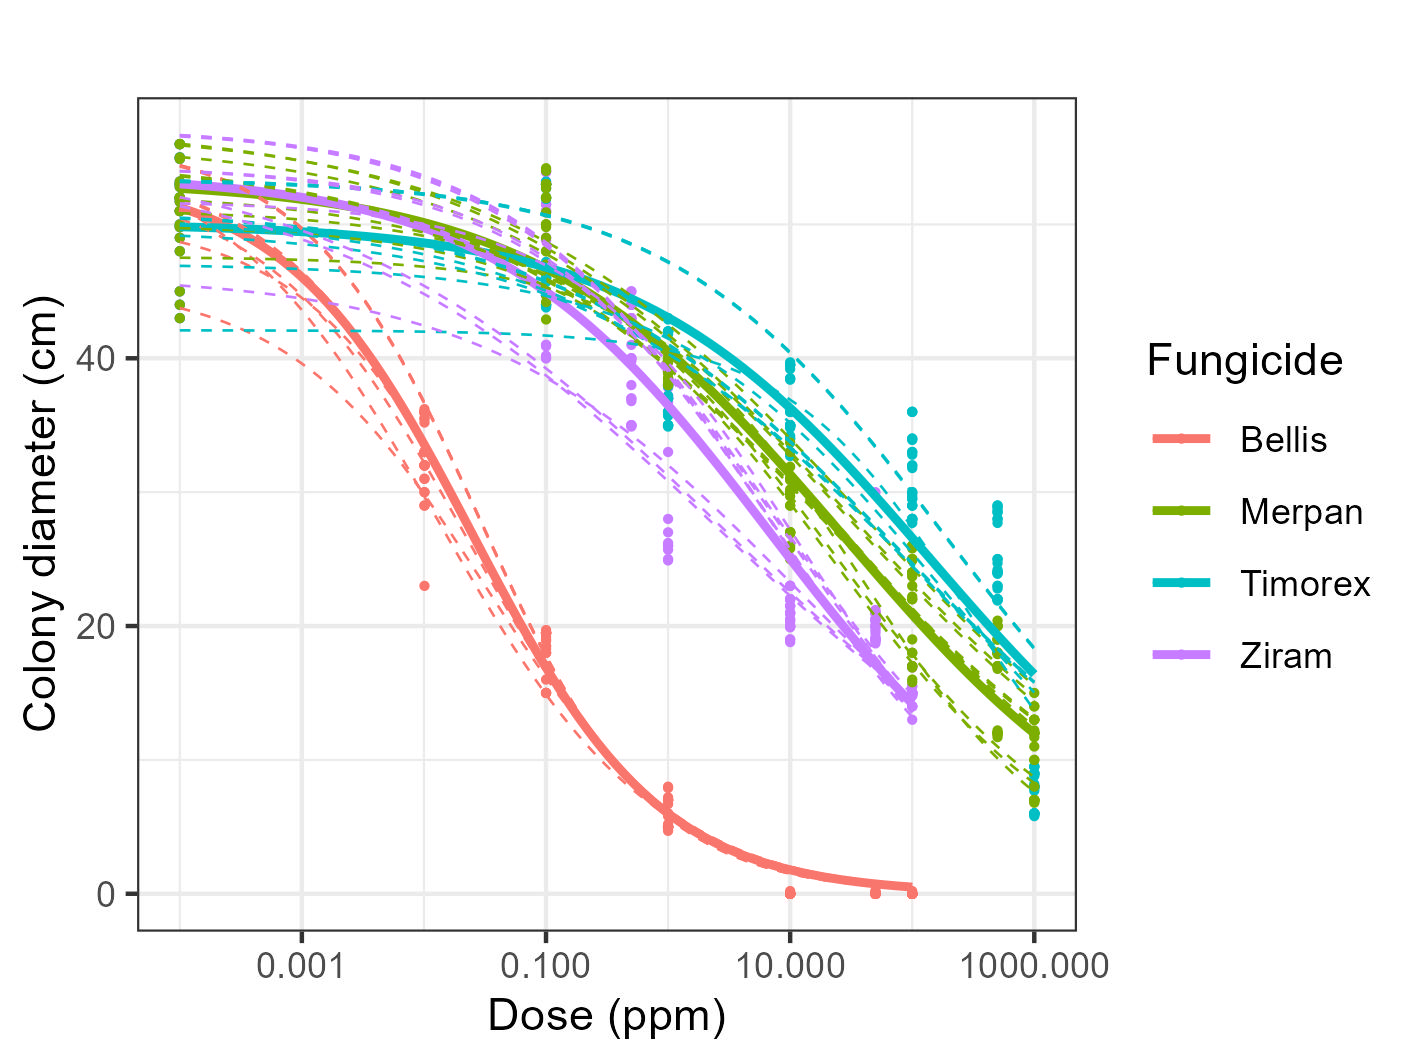
\includegraphics{plots/mg_curves.jpg}

}

\caption{Mycelial growth in function of increasing concentration of
fungicides}

\end{figure}

\hypertarget{spore-germination}{%
\section{Spore germination}\label{spore-germination}}

\begin{Shaded}
\begin{Highlighting}[]
\NormalTok{germi\_raw }\OtherTok{\textless{}{-}} \FunctionTok{import}\NormalTok{(}\StringTok{"data/germination.csv"}\NormalTok{, }\AttributeTok{dec=}\StringTok{","}\NormalTok{)}
\NormalTok{germi\_dat }\OtherTok{\textless{}{-}}\NormalTok{ germi\_raw }\SpecialCharTok{\%\textgreater{}\%} 
  \FunctionTok{mutate\_at}\NormalTok{(}\FunctionTok{vars}\NormalTok{(dose), as.numeric) }\SpecialCharTok{\%\textgreater{}\%} 
  \FunctionTok{mutate\_at}\NormalTok{(}\FunctionTok{vars}\NormalTok{(fungicide, strain, repetition, replicate), as.factor) }\SpecialCharTok{\%\textgreater{}\%} 
  \FunctionTok{mutate}\NormalTok{(}\AttributeTok{curve\_id =} \FunctionTok{interaction}\NormalTok{(fungicide}\SpecialCharTok{:}\NormalTok{strain}\SpecialCharTok{:}\NormalTok{repetition)) }\SpecialCharTok{\%\textgreater{}\%} 
  \FunctionTok{mutate}\NormalTok{(}\AttributeTok{dose\_ =}\NormalTok{ dose}\FloatTok{+0.0001}\NormalTok{)}
\end{Highlighting}
\end{Shaded}

Data structure

\begin{Shaded}
\begin{Highlighting}[]
\FunctionTok{ftable}\NormalTok{(}\FunctionTok{xtabs}\NormalTok{(}\FunctionTok{complete.cases}\NormalTok{(germination\_percent)}\SpecialCharTok{\textasciitilde{}}\NormalTok{fungicide}\SpecialCharTok{+}\NormalTok{dose}\SpecialCharTok{+}\NormalTok{strain , }\AttributeTok{data=}\NormalTok{germi\_dat))}
\end{Highlighting}
\end{Shaded}

\begin{verbatim}
               strain S20 S23 S8
fungicide dose                  
Bellis    0             6   6  6
          0.1           6   6  6
          1             6   6  6
          10            6   6  6
          50            6   6  6
          100           6   6  6
          500           0   0  0
          1000          0   0  0
Merpan    0             6   6  6
          0.1           6   6  6
          1             6   6  6
          10            6   6  6
          50            0   0  0
          100           6   6  6
          500           6   6  6
          1000          6   6  6
Timorex   0             6   6  6
          0.1           6   6  6
          1             6   6  6
          10            6   6  6
          50            0   0  0
          100           6   6  6
          500           6   6  6
          1000          6   6  6
Ziram     0             6   6  6
          0.1           6   6  6
          1             6   6  6
          10            6   6  6
          50            6   6  6
          100           6   6  6
          500           0   0  0
          1000          0   0  0
\end{verbatim}

\begin{Shaded}
\begin{Highlighting}[]
\FunctionTok{str}\NormalTok{(germi\_dat)}
\end{Highlighting}
\end{Shaded}

\begin{verbatim}
'data.frame':   468 obs. of  12 variables:
 $ fungicide             : Factor w/ 4 levels "Bellis","Merpan",..: 1 1 1 1 1 1 1 1 1 1 ...
 $ strain                : Factor w/ 3 levels "S20","S23","S8": 2 2 2 1 1 1 3 3 3 2 ...
 $ repetition            : Factor w/ 2 levels "1","2": 1 1 1 1 1 1 1 1 1 1 ...
 $ replicate             : Factor w/ 3 levels "1","2","3": 1 2 3 1 2 3 1 2 3 1 ...
 $ dose                  : num  100 100 100 100 100 100 100 100 100 50 ...
 $ germinated_conidia    : int  0 0 0 0 0 0 0 0 0 0 ...
 $ total_conida          : int  100 100 100 100 100 100 100 100 100 100 ...
 $ non_germinated_conidia: int  100 100 100 100 100 100 100 100 100 100 ...
 $ inhibition_perc       : int  100 100 100 100 100 100 100 100 100 100 ...
 $ germination_percent   : int  0 0 0 0 0 0 0 0 0 0 ...
 $ curve_id              : Factor w/ 24 levels "Bellis:S20:1",..: 3 3 3 1 1 1 5 5 5 3 ...
 $ dose_                 : num  100 100 100 100 100 ...
\end{verbatim}

Dose-response curves fitting by meta-analysis approach

\begin{Shaded}
\begin{Highlighting}[]
\NormalTok{mod\_germ }\OtherTok{\textless{}{-}} \FunctionTok{metadrm}\NormalTok{(germination\_percent }\SpecialCharTok{\textasciitilde{}}\NormalTok{ dose\_, }
               \AttributeTok{data=}\NormalTok{germi\_dat,}
               \AttributeTok{fct=}\FunctionTok{LL.3}\NormalTok{(),}
               \AttributeTok{ind=}\NormalTok{curve\_id,}
               \AttributeTok{cid2=}\NormalTok{fungicide,}
               \AttributeTok{struct=}\StringTok{"UN"}\NormalTok{)}
\FunctionTok{save}\NormalTok{(mod\_germ, }\AttributeTok{file=} \StringTok{"models/invitro\_germ.rds"}\NormalTok{)}
\end{Highlighting}
\end{Shaded}

\begin{Shaded}
\begin{Highlighting}[]
\FunctionTok{load}\NormalTok{(}\StringTok{"models/invitro\_germ.rds"}\NormalTok{)}
\FunctionTok{summary}\NormalTok{(mod\_germ) }
\end{Highlighting}
\end{Shaded}

\begin{verbatim}

Two-stage meta-analysis dose-response model
Model fitted: Log-logistic (ED50 as parameter) with lower limit at 0

Call:
metadrm(formula = germination_percent ~ dose_, fct = LL.3(), 
    ind = curve_id, data = germi_dat, cid2 = fungicide, struct = "UN")

Variance estimates:
            estim    sqrt
tau^2.1    0.0024  0.0494
tau^2.2    0.0063  0.0792
tau^2.3    0.0001  0.0090

               rho.b:(I  rho.d:(I  rho.e:(I
b:(Intercept)         1    1.0000    1.0000
d:(Intercept)    1.0000         1    1.0000
e:(Intercept)    1.0000    1.0000         1


Coefficients:
             Estimate     Std.Err  t value              Pr(>|t|)    
b:Bellis    1.0898626   0.0854167  12.7594 < 0.00000000000000022 ***
b:Merpan    1.3070417   0.0560275  23.3286 < 0.00000000000000022 ***
b:Timorex   1.0749724   0.1249763   8.6014     0.000000000004650 ***
b:Ziram     0.6145974   0.0415450  14.7935 < 0.00000000000000022 ***
d:Bellis   99.8992681   0.2360299 423.2484 < 0.00000000000000022 ***
d:Merpan   97.9883814   0.5305522 184.6913 < 0.00000000000000022 ***
d:Timorex  97.6597656   1.7236343  56.6592 < 0.00000000000000022 ***
d:Ziram    99.0543330   2.0387322  48.5862 < 0.00000000000000022 ***
e:Bellis    0.0231700   0.0051014   4.5419     0.000027438625743 ***
e:Merpan    1.1355696   0.0241592  47.0036 < 0.00000000000000022 ***
e:Timorex 289.0283519  34.0651922   8.4846     0.000000000007338 ***
e:Ziram     0.1557700   0.0270433   5.7600     0.000000308016186 ***
---
Signif. codes:  0 '***' 0.001 '**' 0.01 '*' 0.05 '.' 0.1 ' ' 1
\end{verbatim}

EC50´s Estimates

\begin{Shaded}
\begin{Highlighting}[]
\NormalTok{ec50s\_g }\OtherTok{\textless{}{-}} \FunctionTok{ED}\NormalTok{(mod\_germ, }\AttributeTok{respLev=}\FunctionTok{c}\NormalTok{(}\DecValTok{50}\NormalTok{)) }\SpecialCharTok{\%\textgreater{}\%} \FunctionTok{as.data.frame}\NormalTok{()}
\end{Highlighting}
\end{Shaded}

\begin{verbatim}

Estimated effective doses

                Estimate  Std. Error
e:Bellis:50    0.0231700   0.0051014
e:Merpan:50    1.1355696   0.0241592
e:Timorex:50 289.0283519  34.0651922
e:Ziram:50     0.1557700   0.0270433
\end{verbatim}

\begin{Shaded}
\begin{Highlighting}[]
\NormalTok{ec50s\_g}
\end{Highlighting}
\end{Shaded}

\begin{verbatim}
                 Estimate   Std. Error
e:Bellis:50    0.02317004  0.005101351
e:Merpan:50    1.13556964  0.024159210
e:Timorex:50 289.02835194 34.065192159
e:Ziram:50     0.15577000  0.027043327
\end{verbatim}

\begin{Shaded}
\begin{Highlighting}[]
\NormalTok{germ\_comp }\OtherTok{\textless{}{-}} \FunctionTok{EDcomp}\NormalTok{(mod\_germ, }
       \AttributeTok{percVec=}\FunctionTok{c}\NormalTok{(}\DecValTok{50}\NormalTok{), }
       \AttributeTok{percMat=}\FunctionTok{rbind}\NormalTok{(}\FunctionTok{c}\NormalTok{(}\DecValTok{1}\NormalTok{,}\DecValTok{1}\NormalTok{,}\DecValTok{1}\NormalTok{,}\DecValTok{1}\NormalTok{)), }
       \AttributeTok{interval=}\StringTok{"fieller"}\NormalTok{)  }\SpecialCharTok{\%\textgreater{}\%} 
\NormalTok{    data.frame }\SpecialCharTok{\%\textgreater{}\%} 
  \FunctionTok{rownames\_to\_column}\NormalTok{(}\StringTok{"comp"}\NormalTok{) }\SpecialCharTok{\%\textgreater{}\%}
  \FunctionTok{rowwise}\NormalTok{() }\SpecialCharTok{\%\textgreater{}\%} 
  \FunctionTok{mutate}\NormalTok{(}\AttributeTok{relative\_to\_one =} \FunctionTok{f}\NormalTok{(Lower, Upper, }\DecValTok{1}\NormalTok{))}
\end{Highlighting}
\end{Shaded}

\begin{verbatim}

Estimated ratios of effect doses

                           Estimate          Lower          Upper
Bellis/Merpan:50/50     0.020403889    0.011404798    0.029477018
Bellis/Timorex:50/50    0.000080165    0.000043407    0.000126360
Bellis/Ziram:50/50      0.148745178    0.077874246    0.260413050
Merpan/Timorex:50/50    0.003928921    0.003164387    0.005155910
Merpan/Ziram:50/50      7.290040642    5.392013944   11.187536191
Timorex/Ziram:50/50  1855.481470394 1241.326870777 2978.546457196
\end{verbatim}

\begin{Shaded}
\begin{Highlighting}[]
\NormalTok{germ\_comp}
\end{Highlighting}
\end{Shaded}

\begin{verbatim}
# A tibble: 6 x 5
# Rowwise: 
  comp                     Estimate        Lower       Upper relative_to_one
  <chr>                       <dbl>        <dbl>       <dbl> <chr>          
1 Bellis/Merpan:50/50     0.0204       0.0114       0.0295   below          
2 Bellis/Timorex:50/50    0.0000802    0.0000434    0.000126 below          
3 Bellis/Ziram:50/50      0.149        0.0779       0.260    below          
4 Merpan/Timorex:50/50    0.00393      0.00316      0.00516  below          
5 Merpan/Ziram:50/50      7.29         5.39        11.2      above          
6 Timorex/Ziram:50/50  1855.        1241.        2979.       above          
\end{verbatim}

\begin{Shaded}
\begin{Highlighting}[]
\NormalTok{coef\_mod\_germ }\OtherTok{\textless{}{-}} \FunctionTok{summary}\NormalTok{(mod\_germ) }\SpecialCharTok{\%\textgreater{}\%}\NormalTok{ data.frame }\SpecialCharTok{\%\textgreater{}\%} 
    \FunctionTok{rownames\_to\_column}\NormalTok{(}\StringTok{"param"}\NormalTok{)  }\SpecialCharTok{\%\textgreater{}\%} 
  \FunctionTok{separate}\NormalTok{(param, }\FunctionTok{c}\NormalTok{(}\StringTok{"param"}\NormalTok{, }\StringTok{"fungicide"}\NormalTok{))}
\end{Highlighting}
\end{Shaded}

\begin{verbatim}

Two-stage meta-analysis dose-response model
Model fitted: Log-logistic (ED50 as parameter) with lower limit at 0

Call:
metadrm(formula = germination_percent ~ dose_, fct = LL.3(), 
    ind = curve_id, data = germi_dat, cid2 = fungicide, struct = "UN")

Variance estimates:
            estim    sqrt
tau^2.1    0.0024  0.0494
tau^2.2    0.0063  0.0792
tau^2.3    0.0001  0.0090

               rho.b:(I  rho.d:(I  rho.e:(I
b:(Intercept)         1    1.0000    1.0000
d:(Intercept)    1.0000         1    1.0000
e:(Intercept)    1.0000    1.0000         1


Coefficients:
             Estimate     Std.Err  t value              Pr(>|t|)    
b:Bellis    1.0898626   0.0854167  12.7594 < 0.00000000000000022 ***
b:Merpan    1.3070417   0.0560275  23.3286 < 0.00000000000000022 ***
b:Timorex   1.0749724   0.1249763   8.6014     0.000000000004650 ***
b:Ziram     0.6145974   0.0415450  14.7935 < 0.00000000000000022 ***
d:Bellis   99.8992681   0.2360299 423.2484 < 0.00000000000000022 ***
d:Merpan   97.9883814   0.5305522 184.6913 < 0.00000000000000022 ***
d:Timorex  97.6597656   1.7236343  56.6592 < 0.00000000000000022 ***
d:Ziram    99.0543330   2.0387322  48.5862 < 0.00000000000000022 ***
e:Bellis    0.0231700   0.0051014   4.5419     0.000027438625743 ***
e:Merpan    1.1355696   0.0241592  47.0036 < 0.00000000000000022 ***
e:Timorex 289.0283519  34.0651922   8.4846     0.000000000007338 ***
e:Ziram     0.1557700   0.0270433   5.7600     0.000000308016186 ***
---
Signif. codes:  0 '***' 0.001 '**' 0.01 '*' 0.05 '.' 0.1 ' ' 1
\end{verbatim}

\begin{Shaded}
\begin{Highlighting}[]
\CommentTok{\# ec50\_germ \textless{}{-} coef\_mod\_germ \%\textgreater{}\% filter(param=="e") }
\CommentTok{\# ec50\_germ}
\end{Highlighting}
\end{Shaded}

\begin{Shaded}
\begin{Highlighting}[]
\NormalTok{germ\_comp }\SpecialCharTok{\%\textgreater{}\%} 
  \FunctionTok{ggplot}\NormalTok{()}\SpecialCharTok{+} 
  \FunctionTok{aes}\NormalTok{(}\AttributeTok{x=}\NormalTok{comp, }\AttributeTok{y=}\NormalTok{Estimate) }\SpecialCharTok{+} 
  \FunctionTok{geom\_pointrange}\NormalTok{(}\FunctionTok{aes}\NormalTok{(}\AttributeTok{ymin =}\NormalTok{ Lower, }\AttributeTok{ymax =}\NormalTok{ Upper, }\AttributeTok{col=}\NormalTok{relative\_to\_one))}\SpecialCharTok{+}     
  \FunctionTok{geom\_hline}\NormalTok{(}\AttributeTok{yintercept =} \DecValTok{1}\NormalTok{, }\AttributeTok{linetype=}\DecValTok{2}\NormalTok{)}\SpecialCharTok{+}
  \FunctionTok{coord\_flip}\NormalTok{() }\SpecialCharTok{+} 
  \FunctionTok{labs}\NormalTok{(}\AttributeTok{col=}\StringTok{"Relative to 1"}\NormalTok{)}
\end{Highlighting}
\end{Shaded}

\begin{Shaded}
\begin{Highlighting}[]
\NormalTok{germi\_dat }\SpecialCharTok{\%\textgreater{}\%} 
  \FunctionTok{ggplot}\NormalTok{()}\SpecialCharTok{+}
  \FunctionTok{aes}\NormalTok{(}\AttributeTok{x=}\NormalTok{dose}\FloatTok{+0.0001}\NormalTok{, }\AttributeTok{y=}\NormalTok{germination\_percent, }\AttributeTok{col=}\NormalTok{fungicide) }\SpecialCharTok{+}
  \FunctionTok{scale\_x\_log10}\NormalTok{() }\SpecialCharTok{+}
  \FunctionTok{geom\_point}\NormalTok{(}\AttributeTok{size=}\DecValTok{1}\NormalTok{) }\SpecialCharTok{+} 
  \FunctionTok{geom\_smooth}\NormalTok{(}\AttributeTok{method =}\NormalTok{ drm, }
              \AttributeTok{method.args =} \FunctionTok{list}\NormalTok{(}\AttributeTok{fct =} \FunctionTok{L.3}\NormalTok{()), }\AttributeTok{se =}\NormalTok{ F) }\SpecialCharTok{+}  
  \FunctionTok{geom\_smooth}\NormalTok{(}\FunctionTok{aes}\NormalTok{(}\AttributeTok{group=}\NormalTok{curve\_id), }\AttributeTok{size=}\NormalTok{.}\DecValTok{3}\NormalTok{, }\AttributeTok{linetype=}\DecValTok{2}\NormalTok{,  }
              \AttributeTok{method =}\NormalTok{ drm, }
              \AttributeTok{method.args =} \FunctionTok{list}\NormalTok{(}\AttributeTok{fct =} \FunctionTok{L.3}\NormalTok{()), }\AttributeTok{se =}\NormalTok{ F) }\SpecialCharTok{+}
  \FunctionTok{labs}\NormalTok{(}\AttributeTok{title=} \StringTok{""}\NormalTok{, }\AttributeTok{x =} \StringTok{"Dose (ppm)"}\NormalTok{,  }\AttributeTok{y =} \StringTok{"Germination (\%)"}\NormalTok{, }\AttributeTok{col=} \StringTok{"Fungicide"}\NormalTok{)  }\SpecialCharTok{+}
  \FunctionTok{theme\_bw}\NormalTok{(}\AttributeTok{base\_family=}\DecValTok{12}\NormalTok{)}
\end{Highlighting}
\end{Shaded}

\begin{Shaded}
\begin{Highlighting}[]
\FunctionTok{ggsave}\NormalTok{(}\FunctionTok{last\_plot}\NormalTok{(), }\AttributeTok{file=}\StringTok{"plots/germi\_curves.jpg"}\NormalTok{, }\AttributeTok{width =} \DecValTok{8}\NormalTok{, }\AttributeTok{height =} \DecValTok{6}\NormalTok{, }\AttributeTok{units =} \StringTok{"cm"}\NormalTok{, }\AttributeTok{scale=}\FloatTok{1.5}\NormalTok{, }\AttributeTok{dpi =} \DecValTok{300}\NormalTok{)}
\end{Highlighting}
\end{Shaded}

\begin{figure}

{\centering 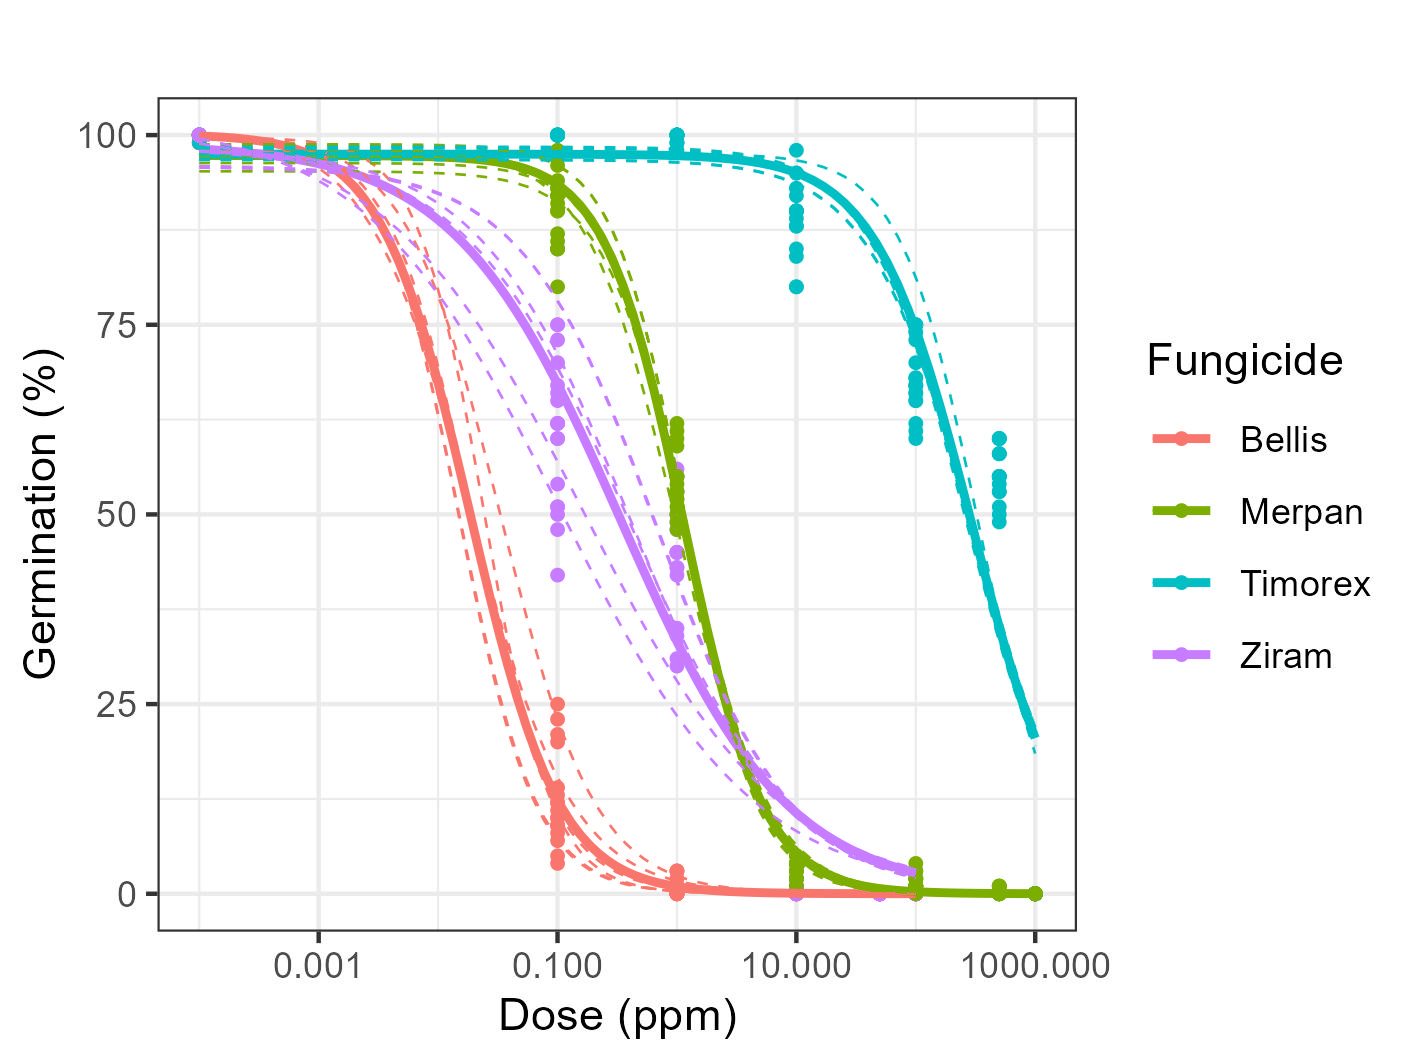
\includegraphics{plots/germi_curves.jpg}

}

\caption{Inhibition of conidial germination}

\end{figure}

\bookmarksetup{startatroot}

\hypertarget{bioassays-in-fruit}{%
\chapter{Bioassays in fruit}\label{bioassays-in-fruit}}

\begin{Shaded}
\begin{Highlighting}[]
\FunctionTok{source}\NormalTok{(here}\SpecialCharTok{::}\FunctionTok{here}\NormalTok{(}\StringTok{"setup.R"}\NormalTok{))}
\end{Highlighting}
\end{Shaded}

\begin{verbatim}
[conflicted] Will prefer dplyr::filter over any other package.
[conflicted] Will prefer dplyr::select over any other package.
\end{verbatim}

\begin{Shaded}
\begin{Highlighting}[]
\FunctionTok{library}\NormalTok{(lme4)}
\FunctionTok{library}\NormalTok{(glmmTMB)}
\FunctionTok{library}\NormalTok{(DHARMa)}
\end{Highlighting}
\end{Shaded}

\begin{verbatim}
This is DHARMa 0.4.6. For overview type '?DHARMa'. For recent changes, type news(package = 'DHARMa')
\end{verbatim}

\begin{Shaded}
\begin{Highlighting}[]
\FunctionTok{theme\_set}\NormalTok{(}\FunctionTok{theme\_bw}\NormalTok{(}\AttributeTok{base\_size=}\DecValTok{12}\NormalTok{))}
\end{Highlighting}
\end{Shaded}

\begin{Shaded}
\begin{Highlighting}[]
\NormalTok{dat }\OtherTok{\textless{}{-}}\NormalTok{ rio}\SpecialCharTok{::}\FunctionTok{import}\NormalTok{(}\StringTok{"data/bioassay\_data.csv"}\NormalTok{) }\SpecialCharTok{\%\textgreater{}\%}
  \FunctionTok{mutate\_at}\NormalTok{(}\FunctionTok{vars}\NormalTok{(fungicide, repetition, day, replicate, fruit), as.factor) }\SpecialCharTok{\%\textgreater{}\%} 
  \FunctionTok{mutate}\NormalTok{(}\AttributeTok{fungicide=}\FunctionTok{fct\_relevel}\NormalTok{(fungicide, }\StringTok{"control"}\NormalTok{))}
\end{Highlighting}
\end{Shaded}

Data structure

\begin{Shaded}
\begin{Highlighting}[]
\FunctionTok{ftable}\NormalTok{(}\FunctionTok{xtabs}\NormalTok{(}\SpecialCharTok{\textasciitilde{}}\NormalTok{ fungicide }\SpecialCharTok{+}\NormalTok{ day }\SpecialCharTok{+}\NormalTok{ repetition }\SpecialCharTok{+}\NormalTok{ replicate, dat))}
\end{Highlighting}
\end{Shaded}

\begin{verbatim}
                         replicate 1 2 3 4
fungicide day repetition                  
control   1   1                    5 5 5 5
              2                    5 5 5 5
          7   1                    5 5 5 5
              2                    5 5 5 5
          15  1                    5 5 5 5
              2                    5 5 5 5
Bellis    1   1                    5 5 5 5
              2                    5 5 5 5
          7   1                    5 5 5 5
              2                    5 5 5 5
          15  1                    5 5 5 5
              2                    5 5 5 5
Merpan    1   1                    5 5 5 5
              2                    5 5 5 5
          7   1                    5 5 5 5
              2                    5 5 5 5
          15  1                    5 5 5 5
              2                    5 5 5 5
Timorex   1   1                    5 5 5 5
              2                    5 5 5 5
          7   1                    5 5 5 5
              2                    5 5 5 5
          15  1                    5 5 5 5
              2                    5 5 5 5
Ziram     1   1                    5 5 5 5
              2                    5 5 5 5
          7   1                    5 5 5 5
              2                    5 5 5 5
          15  1                    5 5 5 5
              2                    5 5 5 5
\end{verbatim}

\begin{Shaded}
\begin{Highlighting}[]
\NormalTok{dat }\SpecialCharTok{\%\textgreater{}\%}\NormalTok{ str}
\end{Highlighting}
\end{Shaded}

\begin{verbatim}
'data.frame':   600 obs. of  6 variables:
 $ fungicide      : Factor w/ 5 levels "control","Bellis",..: 2 2 2 2 2 2 2 2 2 2 ...
 $ repetition     : Factor w/ 2 levels "1","2": 1 1 1 1 1 1 1 1 1 1 ...
 $ day            : Factor w/ 3 levels "1","7","15": 1 1 1 1 1 1 1 1 1 1 ...
 $ replicate      : Factor w/ 4 levels "1","2","3","4": 1 1 1 1 1 2 2 2 2 2 ...
 $ fruit          : Factor w/ 5 levels "1","2","3","4",..: 1 2 3 4 5 1 2 3 4 5 ...
 $ spots_per_fruit: int  1 0 0 0 0 0 0 0 0 0 ...
\end{verbatim}

\hypertarget{preventive-treatments}{%
\section{Preventive treatments}\label{preventive-treatments}}

Disease severity (spots per fruit)

\begin{Shaded}
\begin{Highlighting}[]
\NormalTok{dat }\SpecialCharTok{\%\textgreater{}\%} 
  \FunctionTok{ggplot}\NormalTok{() }\SpecialCharTok{+} 
  \FunctionTok{aes}\NormalTok{(}\AttributeTok{x=}\NormalTok{day, }\AttributeTok{y=}\NormalTok{spots\_per\_fruit) }\SpecialCharTok{+} 
  \FunctionTok{geom\_jitter}\NormalTok{(}\AttributeTok{width=}\NormalTok{.}\DecValTok{2}\NormalTok{, }\AttributeTok{col=}\DecValTok{2}\NormalTok{, }\AttributeTok{alpha=}\NormalTok{.}\DecValTok{5}\NormalTok{) }\SpecialCharTok{+} 
  \FunctionTok{geom\_boxplot}\NormalTok{(}\AttributeTok{width=}\NormalTok{.}\DecValTok{5}\NormalTok{, }\AttributeTok{alpha=}\NormalTok{.}\DecValTok{1}\NormalTok{) }\SpecialCharTok{+} 
  \FunctionTok{labs}\NormalTok{(}\AttributeTok{x=}\StringTok{"Fungicide timing (days after inoculation)"}\NormalTok{, }
       \AttributeTok{y=}\StringTok{"Severity (spots per fruit)"}\NormalTok{) }\SpecialCharTok{+} 
  \FunctionTok{facet\_grid}\NormalTok{(repetition}\SpecialCharTok{\textasciitilde{}}\NormalTok{fungicide)}
\end{Highlighting}
\end{Shaded}

\begin{figure}[H]

{\centering 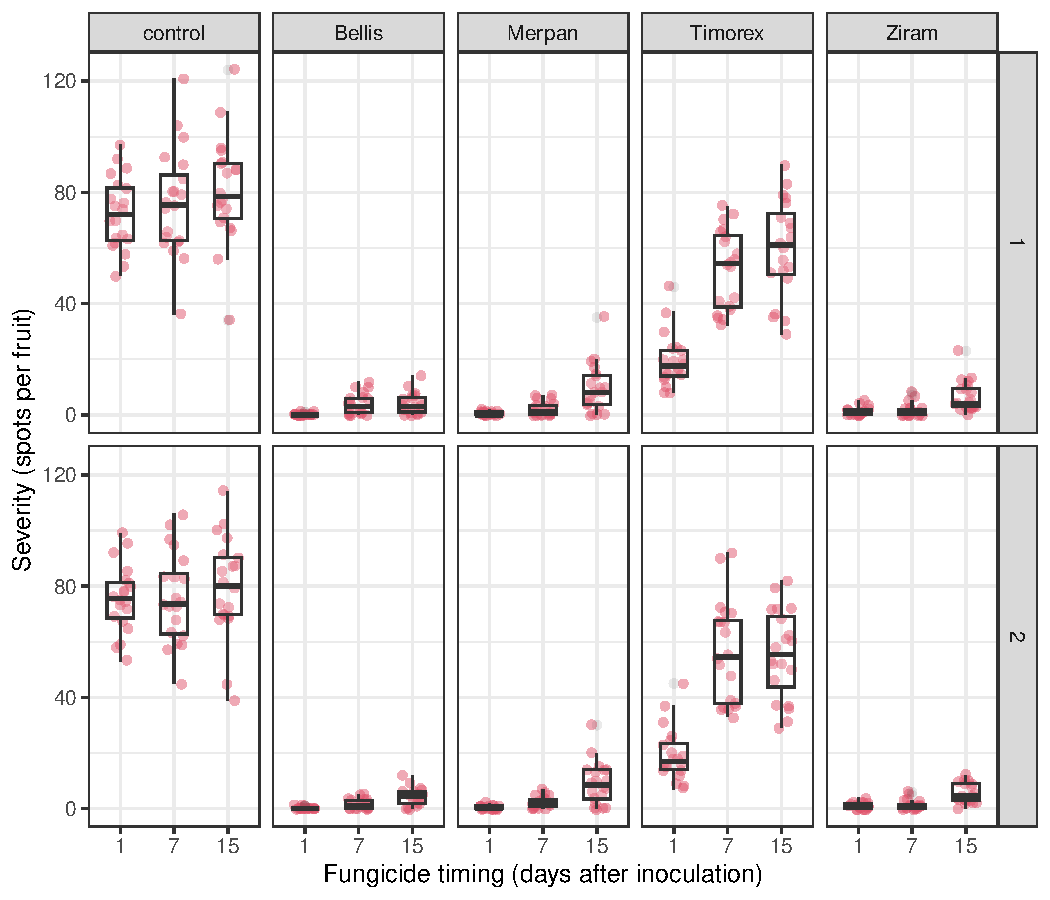
\includegraphics{bioassay_files/figure-pdf/unnamed-chunk-5-1.pdf}

}

\end{figure}

\begin{Shaded}
\begin{Highlighting}[]
\NormalTok{dat }\SpecialCharTok{\%\textgreater{}\%} 
  \FunctionTok{count}\NormalTok{(spots\_per\_fruit) }\SpecialCharTok{\%\textgreater{}\%} 
  \FunctionTok{ggplot}\NormalTok{() }\SpecialCharTok{+} 
  \FunctionTok{aes}\NormalTok{(}\AttributeTok{x=}\NormalTok{spots\_per\_fruit, }\AttributeTok{y=}\NormalTok{n) }\SpecialCharTok{+} 
  \FunctionTok{geom\_col}\NormalTok{()}
\end{Highlighting}
\end{Shaded}

\begin{figure}[H]

{\centering 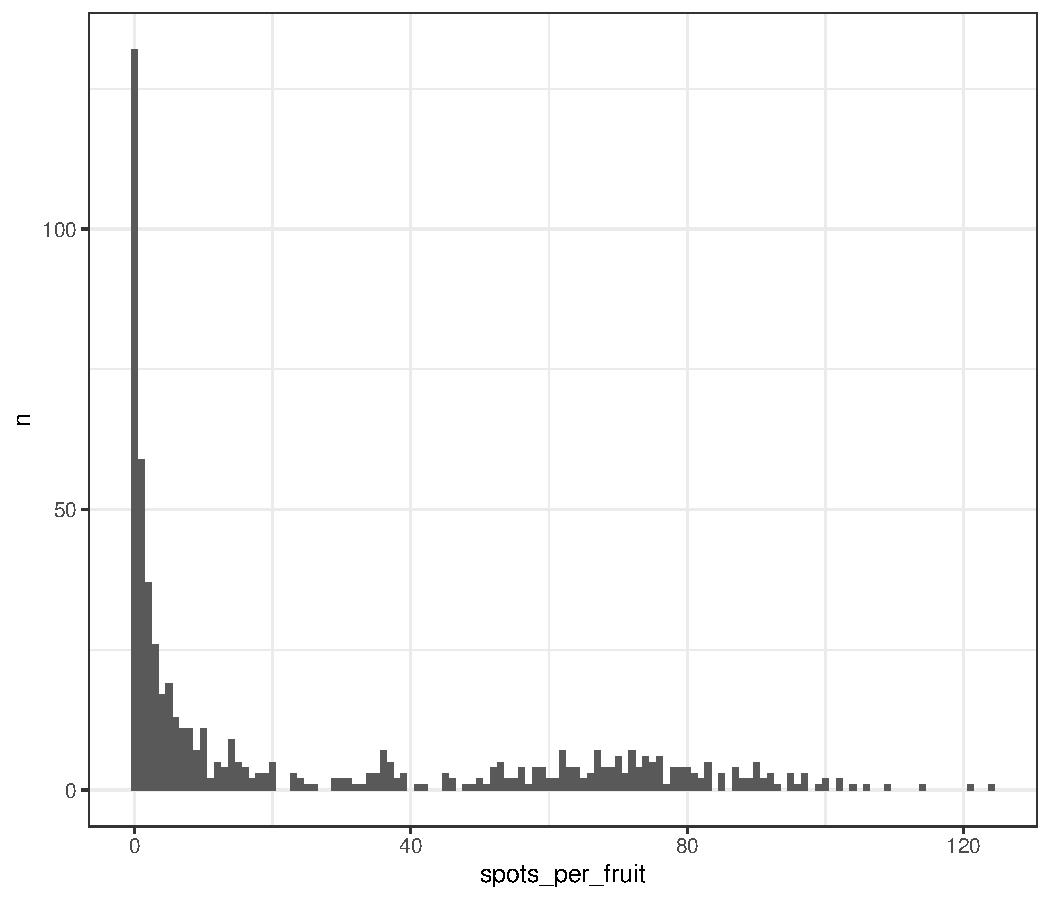
\includegraphics{bioassay_files/figure-pdf/unnamed-chunk-6-1.pdf}

}

\end{figure}

Model fitting

\begin{Shaded}
\begin{Highlighting}[]
\CommentTok{\# https://glmmtmb.github.io/glmmTMB/articles/glmmTMB.pdf}
\NormalTok{fit\_zipoisson\_prev }\OtherTok{\textless{}{-}} \FunctionTok{glmmTMB}\NormalTok{(spots\_per\_fruit}\SpecialCharTok{\textasciitilde{}}\NormalTok{fungicide}\SpecialCharTok{*}\NormalTok{day }\SpecialCharTok{+}
\NormalTok{                           (}\DecValTok{1}\SpecialCharTok{|}\NormalTok{repetition}\SpecialCharTok{/}\NormalTok{replicate),}
               \AttributeTok{ziformula =} \SpecialCharTok{\textasciitilde{}}\DecValTok{1}\NormalTok{, }\AttributeTok{family =}\NormalTok{ poisson,}
\NormalTok{             dat)}
\end{Highlighting}
\end{Shaded}

\begin{Shaded}
\begin{Highlighting}[]
\NormalTok{fit\_zinbinom\_prev }\OtherTok{\textless{}{-}} \FunctionTok{update}\NormalTok{(fit\_zipoisson\_prev,}\AttributeTok{family=}\NormalTok{nbinom2)}
\NormalTok{fit\_zinbinom1\_prev }\OtherTok{\textless{}{-}} \FunctionTok{update}\NormalTok{(fit\_zipoisson\_prev,}\AttributeTok{family=}\NormalTok{nbinom1)}
\NormalTok{fit\_twediee\_prev }\OtherTok{\textless{}{-}} \FunctionTok{update}\NormalTok{(fit\_zipoisson\_prev,}\AttributeTok{family=}\NormalTok{tweedie)}
\FunctionTok{AIC}\NormalTok{(fit\_zipoisson\_prev,fit\_zinbinom\_prev,fit\_zinbinom1\_prev, fit\_twediee\_prev)}
\end{Highlighting}
\end{Shaded}

\begin{verbatim}
                   df      AIC
fit_zipoisson_prev 18 3890.310
fit_zinbinom_prev  19 3486.965
fit_zinbinom1_prev 19 3419.425
fit_twediee_prev   20 3405.244
\end{verbatim}

Goodness of fit

\begin{Shaded}
\begin{Highlighting}[]
\NormalTok{DHARMa}\SpecialCharTok{::}\FunctionTok{testOverdispersion}\NormalTok{(fit\_twediee\_prev)}
\NormalTok{DHARMa}\SpecialCharTok{::}\FunctionTok{testSimulatedResiduals}\NormalTok{(fit\_twediee\_prev)}
\CommentTok{\# simulateResiduals(fit\_twediee\_prev) \%\textgreater{}\% testResiduals()}
\end{Highlighting}
\end{Shaded}

\begin{Shaded}
\begin{Highlighting}[]
\NormalTok{car}\SpecialCharTok{::}\FunctionTok{Anova}\NormalTok{(fit\_twediee\_prev)}
\end{Highlighting}
\end{Shaded}

\begin{verbatim}
Analysis of Deviance Table (Type II Wald chisquare tests)

Response: spots_per_fruit
                Chisq Df            Pr(>Chisq)    
fungicide     2826.15  4 < 0.00000000000000022 ***
day            148.41  2 < 0.00000000000000022 ***
fungicide:day  327.88  8 < 0.00000000000000022 ***
---
Signif. codes:  0 '***' 0.001 '**' 0.01 '*' 0.05 '.' 0.1 ' ' 1
\end{verbatim}

Treatment means comparison

\begin{Shaded}
\begin{Highlighting}[]
\NormalTok{emm\_prev }\OtherTok{\textless{}{-}} \FunctionTok{emmeans}\NormalTok{(fit\_twediee\_prev, }\SpecialCharTok{\textasciitilde{}}\NormalTok{ fungicide}\SpecialCharTok{|}\NormalTok{day, }\AttributeTok{type=}\StringTok{"response"}\NormalTok{) }
\NormalTok{res\_prev }\OtherTok{\textless{}{-}} \FunctionTok{cld}\NormalTok{(emm\_prev, }\AttributeTok{alpha=}\FloatTok{0.05}\NormalTok{, }\AttributeTok{Letters=}\NormalTok{letters,  }\AttributeTok{type=}\StringTok{"response"}\NormalTok{)}
\NormalTok{res\_prev }\SpecialCharTok{\%\textgreater{}\%} 
   \FunctionTok{mutate}\NormalTok{(}\StringTok{\textasciigrave{}}\AttributeTok{\%Control}\StringTok{\textasciigrave{}}\OtherTok{=}\FunctionTok{abs}\NormalTok{((response}\SpecialCharTok{/}\FunctionTok{filter}\NormalTok{(.,fungicide}\SpecialCharTok{==}\StringTok{"control"}\NormalTok{)}\SpecialCharTok{\%\textgreater{}\%} \FunctionTok{pull}\NormalTok{(response)}\SpecialCharTok{{-}}\DecValTok{1}\NormalTok{)}\SpecialCharTok{*}\DecValTok{100}\NormalTok{)) }
\end{Highlighting}
\end{Shaded}

\begin{verbatim}
   fungicide day   response         SE  df   asymp.LCL  asymp.UCL .group
2     Bellis   1  0.1266087 0.06435246 Inf  0.04675374  0.3428553   a   
3     Merpan   1  0.5055717 0.14652770 Inf  0.28647233  0.8922425   ab  
5      Ziram   1  1.1179829 0.23580319 Inf  0.73943685  1.6903213    b  
4    Timorex   1 19.4414909 1.33246605 Inf 16.99771586 22.2366094     c 
1    control   1 73.8540017 3.22802344 Inf 67.79061416 80.4597161      d
10     Ziram   7  1.4931835 0.28182958 Inf  1.03146361  2.1615857    a  
8     Merpan   7  2.3203471 0.36915475 Inf  1.69875745  3.1693817    a  
7     Bellis   7  2.7964637 0.41667960 Inf  2.08822925  3.7448997    a  
9    Timorex   7 54.1858706 2.60846796 Inf 49.30714307 59.5473271     b 
6    control   7 75.9541403 3.29232755 Inf 69.76780397 82.6890213      c
12    Bellis  15  4.3163835 0.54531743 Inf  3.36962889  5.5291449   a   
15     Ziram  15  6.1277829 0.66068554 Inf  4.96053467  7.5696928   a   
13    Merpan  15 10.2948040 1.26533588 Inf  8.09089887 13.0990376    b  
14   Timorex  15 57.5035175 2.71593663 Inf 52.41933283 63.0808205     c 
11   control  15 79.8718272 3.41023449 Inf 73.45991670 86.8433980      d
    %Control
2  99.828569
3  99.334372
5  98.600279
4  73.675779
1   2.765009
10 98.130525
8  96.858197
7  96.318221
9  32.158970
6   2.843635
12 94.317119
15 92.327980
13 86.060601
14 24.291793
11  0.000000
\end{verbatim}

\begin{Shaded}
\begin{Highlighting}[]
\NormalTok{res\_prev }\SpecialCharTok{\%\textgreater{}\%} 
  \FunctionTok{ggplot}\NormalTok{()}\SpecialCharTok{+}
  \FunctionTok{aes}\NormalTok{(}\AttributeTok{x=}\NormalTok{day, }\AttributeTok{y =}\NormalTok{response)}\SpecialCharTok{+}
  \FunctionTok{geom\_pointrange}\NormalTok{(}\FunctionTok{aes}\NormalTok{(}\AttributeTok{ymin=}\NormalTok{asymp.LCL , }\AttributeTok{ymax=}\NormalTok{asymp.UCL))}\SpecialCharTok{+}
  \FunctionTok{geom\_col}\NormalTok{(}\AttributeTok{alpha=}\NormalTok{.}\DecValTok{2}\NormalTok{, }\AttributeTok{width=}\NormalTok{.}\DecValTok{2}\NormalTok{)}\SpecialCharTok{+}
  \FunctionTok{facet\_wrap}\NormalTok{(}\StringTok{"fungicide"}\NormalTok{)}\SpecialCharTok{+}
    \FunctionTok{labs}\NormalTok{(}\AttributeTok{x=}\StringTok{"Fungicide timing (days before inoculation)"}\NormalTok{, }
         \AttributeTok{y=}\StringTok{"Spots per fruit (counts)"}\NormalTok{)}
\end{Highlighting}
\end{Shaded}

\begin{figure}[H]

{\centering 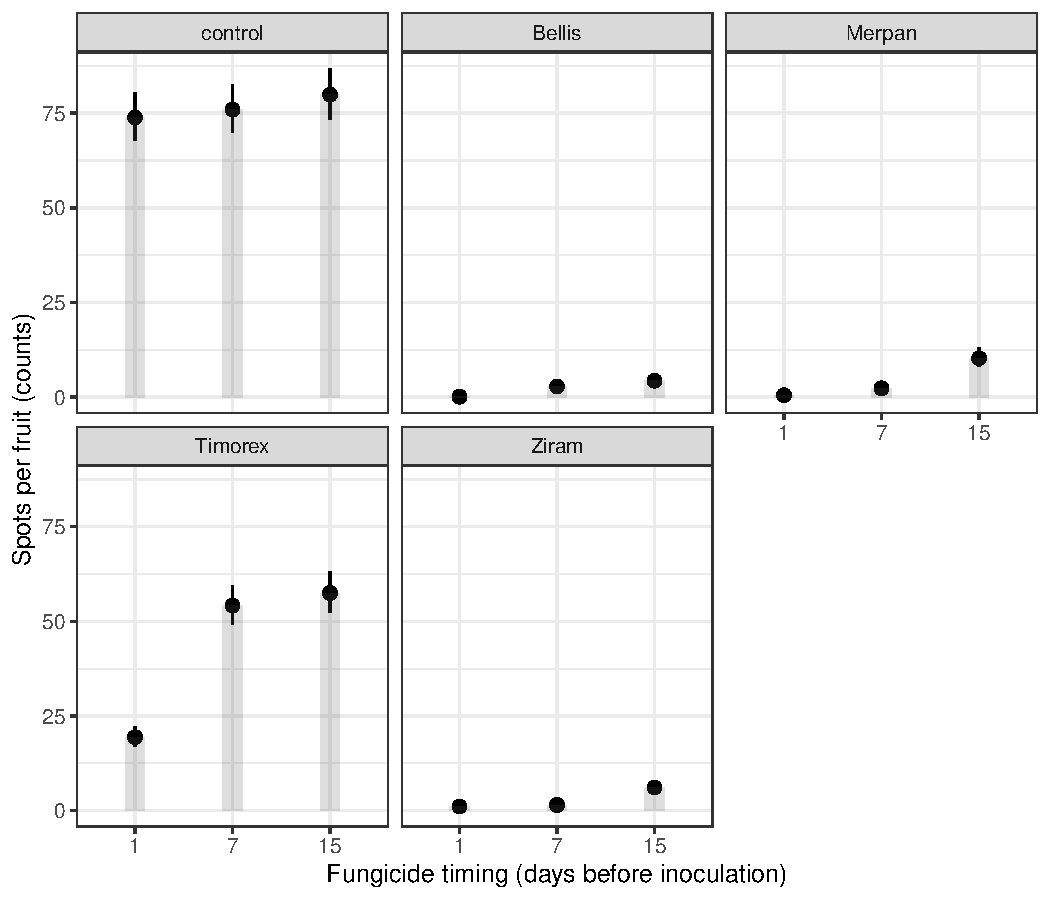
\includegraphics{bioassay_files/figure-pdf/unnamed-chunk-11-1.pdf}

}

\end{figure}

\hypertarget{curative-treatments}{%
\section{Curative treatments}\label{curative-treatments}}

\begin{Shaded}
\begin{Highlighting}[]
\NormalTok{cura }\OtherTok{\textless{}{-}}\NormalTok{ rio}\SpecialCharTok{::}\FunctionTok{import}\NormalTok{(}\StringTok{"data/curative.csv"}\NormalTok{) }\SpecialCharTok{\%\textgreater{}\%} 
   \FunctionTok{mutate\_at}\NormalTok{(}\FunctionTok{vars}\NormalTok{(fungicide, repetition, replicate, fruit), as.factor) }\SpecialCharTok{\%\textgreater{}\%} 
  \FunctionTok{mutate}\NormalTok{(}\AttributeTok{fungicide=}\FunctionTok{fct\_relevel}\NormalTok{(fungicide, }\StringTok{"Control"}\NormalTok{)) }
\end{Highlighting}
\end{Shaded}

Data structure

\begin{Shaded}
\begin{Highlighting}[]
\FunctionTok{ftable}\NormalTok{(}\FunctionTok{xtabs}\NormalTok{(}\SpecialCharTok{\textasciitilde{}}\NormalTok{ fungicide }\SpecialCharTok{+}\NormalTok{ repetition }\SpecialCharTok{+}\NormalTok{ replicate, cura))}
\end{Highlighting}
\end{Shaded}

\begin{verbatim}
                     replicate 1 2 3 4
fungicide repetition                  
Control   1                    5 5 5 5
          2                    5 5 5 5
Bellis    1                    5 5 5 5
          2                    5 5 5 5
Merpan    1                    5 5 5 5
          2                    5 5 5 5
Timorex   1                    5 5 5 5
          2                    5 5 5 5
Ziram     1                    5 5 5 5
          2                    5 5 5 5
\end{verbatim}

\begin{Shaded}
\begin{Highlighting}[]
\NormalTok{cura }\SpecialCharTok{\%\textgreater{}\%}\NormalTok{ str}
\end{Highlighting}
\end{Shaded}

\begin{verbatim}
'data.frame':   200 obs. of  5 variables:
 $ fungicide      : Factor w/ 5 levels "Control","Bellis",..: 1 1 1 1 1 1 1 1 1 1 ...
 $ repetition     : Factor w/ 2 levels "1","2": 1 1 1 1 1 1 1 1 1 1 ...
 $ replicate      : Factor w/ 4 levels "1","2","3","4": 1 1 1 1 1 2 2 2 2 2 ...
 $ fruit          : Factor w/ 5 levels "1","2","3","4",..: 1 2 3 4 5 1 2 3 4 5 ...
 $ spots_per_fruit: int  33 32 40 22 16 16 6 14 41 30 ...
\end{verbatim}

Disease severity (spots per fruit)

\begin{Shaded}
\begin{Highlighting}[]
\NormalTok{cura }\SpecialCharTok{\%\textgreater{}\%} 
  \FunctionTok{ggplot}\NormalTok{() }\SpecialCharTok{+} 
  \FunctionTok{aes}\NormalTok{(}\AttributeTok{x=}\NormalTok{fungicide, }\AttributeTok{y=}\NormalTok{spots\_per\_fruit) }\SpecialCharTok{+} 
  \FunctionTok{geom\_boxplot}\NormalTok{(}\AttributeTok{width=}\NormalTok{.}\DecValTok{5}\NormalTok{) }\SpecialCharTok{+} 
  \FunctionTok{geom\_jitter}\NormalTok{(}\AttributeTok{width=}\NormalTok{.}\DecValTok{2}\NormalTok{, }\AttributeTok{col=}\DecValTok{2}\NormalTok{, }\AttributeTok{alpha=}\NormalTok{.}\DecValTok{5}\NormalTok{) }\SpecialCharTok{+} 
  \FunctionTok{labs}\NormalTok{(}\AttributeTok{x=}\StringTok{"Treatment"}\NormalTok{, }\AttributeTok{y=}\StringTok{"Severity (spots per fruit)"}\NormalTok{) }\SpecialCharTok{+} 
  \FunctionTok{facet\_wrap}\NormalTok{(}\StringTok{"repetition"}\NormalTok{)}
\end{Highlighting}
\end{Shaded}

\begin{figure}[H]

{\centering 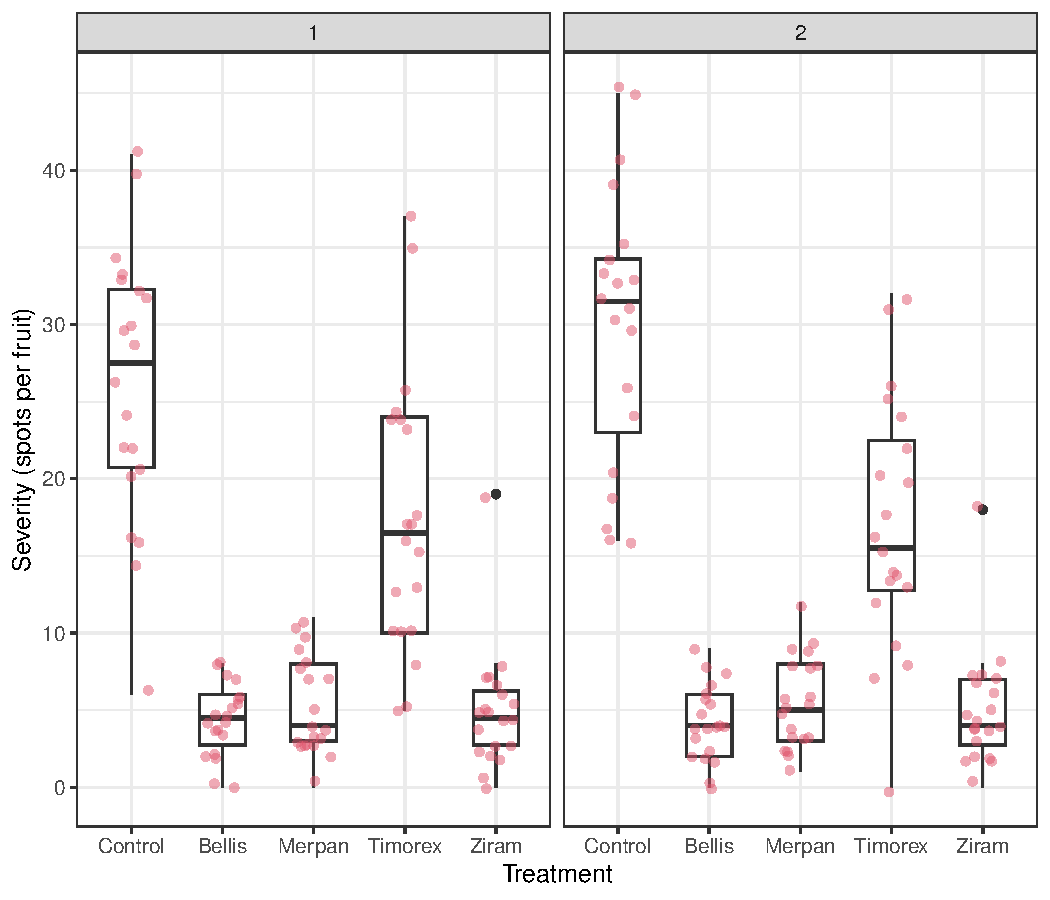
\includegraphics{bioassay_files/figure-pdf/unnamed-chunk-15-1.pdf}

}

\end{figure}

Model fitting

\begin{Shaded}
\begin{Highlighting}[]
\CommentTok{\# https://glmmtmb.github.io/glmmTMB/articles/glmmTMB.pdf}
\NormalTok{fit\_zipoisson\_cur }\OtherTok{\textless{}{-}} \FunctionTok{glmmTMB}\NormalTok{(spots\_per\_fruit}\SpecialCharTok{\textasciitilde{}}\NormalTok{fungicide }\SpecialCharTok{+}
\NormalTok{                               (}\DecValTok{1}\SpecialCharTok{|}\NormalTok{repetition}\SpecialCharTok{/}\NormalTok{replicate),}
                             \AttributeTok{ziformula =} \SpecialCharTok{\textasciitilde{}}\DecValTok{1}\NormalTok{, }
                             \AttributeTok{family =}\NormalTok{ poisson,}\AttributeTok{data =}\NormalTok{ cura)}
\end{Highlighting}
\end{Shaded}

\begin{Shaded}
\begin{Highlighting}[]
\NormalTok{fit\_zinbinom\_cur }\OtherTok{\textless{}{-}} \FunctionTok{update}\NormalTok{(fit\_zipoisson\_cur,}\AttributeTok{family=}\NormalTok{nbinom2)}
\NormalTok{fit\_zinbinom1\_cur }\OtherTok{\textless{}{-}} \FunctionTok{update}\NormalTok{(fit\_zipoisson\_cur,}\AttributeTok{family=}\NormalTok{nbinom1)}
\NormalTok{fit\_twediee\_cur }\OtherTok{\textless{}{-}} \FunctionTok{update}\NormalTok{(fit\_zipoisson\_cur,}\AttributeTok{family=}\NormalTok{tweedie)}
\FunctionTok{AIC}\NormalTok{(fit\_zipoisson\_cur,fit\_zinbinom\_cur,fit\_zinbinom1\_cur, fit\_twediee\_cur)}
\end{Highlighting}
\end{Shaded}

\begin{verbatim}
                  df      AIC
fit_zipoisson_cur  8 1264.879
fit_zinbinom_cur   9 1176.775
fit_zinbinom1_cur  9 1184.694
fit_twediee_cur   10 1179.372
\end{verbatim}

\begin{Shaded}
\begin{Highlighting}[]
\CommentTok{\#               df      AIC}
\CommentTok{\# fit\_zipoisson  8 1270.421}
\CommentTok{\# fit\_zinbinom   9 1176.582}
\CommentTok{\# fit\_zinbinom1  9 1182.421}
\CommentTok{\# fit\_twediee   10 1180.572}
\end{Highlighting}
\end{Shaded}

Goodness of fit

\begin{Shaded}
\begin{Highlighting}[]
\FunctionTok{simulateResiduals}\NormalTok{(fit\_twediee\_cur) }\SpecialCharTok{\%\textgreater{}\%} \FunctionTok{testResiduals}\NormalTok{()}
\end{Highlighting}
\end{Shaded}

\begin{Shaded}
\begin{Highlighting}[]
\NormalTok{car}\SpecialCharTok{::}\FunctionTok{Anova}\NormalTok{(fit\_twediee\_cur)}
\end{Highlighting}
\end{Shaded}

\begin{verbatim}
Analysis of Deviance Table (Type II Wald chisquare tests)

Response: spots_per_fruit
          Chisq Df            Pr(>Chisq)    
fungicide 533.4  4 < 0.00000000000000022 ***
---
Signif. codes:  0 '***' 0.001 '**' 0.01 '*' 0.05 '.' 0.1 ' ' 1
\end{verbatim}

Treatment means comparison

\begin{Shaded}
\begin{Highlighting}[]
\NormalTok{emm\_cura }\OtherTok{\textless{}{-}} \FunctionTok{emmeans}\NormalTok{(fit\_twediee\_cur, }\SpecialCharTok{\textasciitilde{}}\NormalTok{ fungicide, }\AttributeTok{type=}\StringTok{"response"}\NormalTok{) }
\NormalTok{res\_cura }\OtherTok{\textless{}{-}} \FunctionTok{cld}\NormalTok{(emm\_cura, }\AttributeTok{alpha=}\FloatTok{0.05}\NormalTok{, }\AttributeTok{Letters=}\NormalTok{letters,  }\AttributeTok{type=}\StringTok{"response"}\NormalTok{)}
\NormalTok{res\_cura }\SpecialCharTok{\%\textgreater{}\%} 
    \FunctionTok{mutate}\NormalTok{(}\StringTok{\textasciigrave{}}\AttributeTok{\%Control}\StringTok{\textasciigrave{}}\OtherTok{=}\FunctionTok{abs}\NormalTok{((response}\SpecialCharTok{/}\FunctionTok{filter}\NormalTok{(.,fungicide}\SpecialCharTok{==}\StringTok{"Control"}\NormalTok{)}\SpecialCharTok{\%\textgreater{}\%} \FunctionTok{pull}\NormalTok{(response)}\SpecialCharTok{{-}}\DecValTok{1}\NormalTok{)}\SpecialCharTok{*}\DecValTok{100}\NormalTok{)) }
\end{Highlighting}
\end{Shaded}

\begin{verbatim}
  fungicide  response        SE  df asymp.LCL asymp.UCL .group %Control
2    Bellis  4.803382 0.4445747 Inf  4.006495  5.758770    a   82.81883
5     Ziram  5.180715 0.4648248 Inf  4.345283  6.176768    a   81.46916
3    Merpan  5.478331 0.4804890 Inf  4.613089  6.505861    a   80.40462
4   Timorex 17.539752 1.3205836 Inf 15.133372 20.328773     b  37.26226
1   Control 27.957257 1.9647959 Inf 24.359778 32.086015      c  0.00000
\end{verbatim}

\begin{Shaded}
\begin{Highlighting}[]
\NormalTok{res\_cura }\SpecialCharTok{\%\textgreater{}\%} 
  \FunctionTok{ggplot}\NormalTok{()}\SpecialCharTok{+}
  \FunctionTok{aes}\NormalTok{(}\AttributeTok{x=}\NormalTok{fungicide, }\AttributeTok{y =}\NormalTok{response)}\SpecialCharTok{+}
  \FunctionTok{geom\_pointrange}\NormalTok{(}\FunctionTok{aes}\NormalTok{(}\AttributeTok{ymin=}\NormalTok{asymp.LCL , }\AttributeTok{ymax=}\NormalTok{asymp.UCL))}\SpecialCharTok{+}
  \FunctionTok{geom\_col}\NormalTok{(}\AttributeTok{alpha=}\NormalTok{.}\DecValTok{2}\NormalTok{, }\AttributeTok{width=}\NormalTok{.}\DecValTok{2}\NormalTok{)}
\end{Highlighting}
\end{Shaded}

\begin{figure}[H]

{\centering 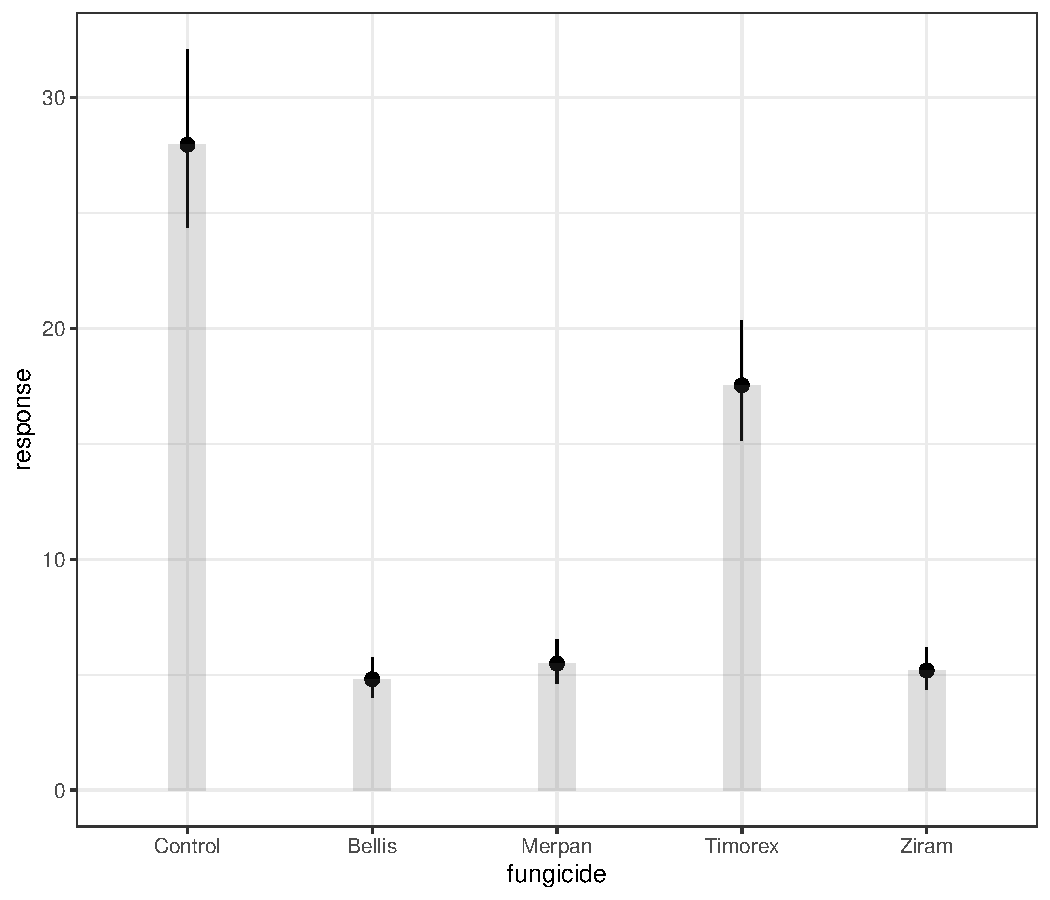
\includegraphics{bioassay_files/figure-pdf/unnamed-chunk-20-1.pdf}

}

\end{figure}

\bookmarksetup{startatroot}

\hypertarget{field-experiments}{%
\chapter{Field experiments}\label{field-experiments}}

\begin{Shaded}
\begin{Highlighting}[]
\FunctionTok{source}\NormalTok{(here}\SpecialCharTok{::}\FunctionTok{here}\NormalTok{(}\StringTok{"setup.R"}\NormalTok{))}
\end{Highlighting}
\end{Shaded}

\begin{verbatim}
[conflicted] Will prefer dplyr::filter over any other package.
[conflicted] Will prefer dplyr::select over any other package.
\end{verbatim}

\begin{Shaded}
\begin{Highlighting}[]
\FunctionTok{library}\NormalTok{(lme4)}
\FunctionTok{theme\_set}\NormalTok{(}\FunctionTok{theme\_bw}\NormalTok{(}\AttributeTok{base\_size=}\DecValTok{12}\NormalTok{))}
\end{Highlighting}
\end{Shaded}

\begin{Shaded}
\begin{Highlighting}[]
\NormalTok{dat }\OtherTok{\textless{}{-}}\NormalTok{ rio}\SpecialCharTok{::}\FunctionTok{import}\NormalTok{(}\StringTok{"data/field.csv"}\NormalTok{) }\SpecialCharTok{\%\textgreater{}\%} 
  \FunctionTok{mutate\_at}\NormalTok{(}\FunctionTok{vars}\NormalTok{(fungicide, season, tree), as.factor) }\SpecialCharTok{\%\textgreater{}\%} 
  \FunctionTok{mutate}\NormalTok{(}\AttributeTok{fungicide=}\FunctionTok{fct\_relevel}\NormalTok{(fungicide, }\StringTok{"Control"}\NormalTok{))}
\FunctionTok{str}\NormalTok{(dat)}
\end{Highlighting}
\end{Shaded}

\begin{verbatim}
'data.frame':   60 obs. of  5 variables:
 $ fungicide: Factor w/ 3 levels "Control","Bellis",..: 1 1 1 1 1 1 1 1 1 1 ...
 $ season   : Factor w/ 2 levels "1","2": 2 2 2 2 2 2 2 2 2 2 ...
 $ tree     : Factor w/ 10 levels "1","2","3","4",..: 1 2 3 4 5 6 7 8 9 10 ...
 $ leaves   : int  250 250 250 250 250 250 250 250 250 250 ...
 $ diseased : int  27 19 26 30 16 40 27 22 19 8 ...
\end{verbatim}

Data structure

\begin{Shaded}
\begin{Highlighting}[]
\FunctionTok{ftable}\NormalTok{(}\FunctionTok{xtabs}\NormalTok{(}\SpecialCharTok{\textasciitilde{}}\NormalTok{ fungicide }\SpecialCharTok{+}\NormalTok{ tree }\SpecialCharTok{+}\NormalTok{ season, dat))}
\end{Highlighting}
\end{Shaded}

\begin{verbatim}
               season 1 2
fungicide tree           
Control   1           1 1
          2           1 1
          3           1 1
          4           1 1
          5           1 1
          6           1 1
          7           1 1
          8           1 1
          9           1 1
          10          1 1
Bellis    1           1 1
          2           1 1
          3           1 1
          4           1 1
          5           1 1
          6           1 1
          7           1 1
          8           1 1
          9           1 1
          10          1 1
Ziram     1           1 1
          2           1 1
          3           1 1
          4           1 1
          5           1 1
          6           1 1
          7           1 1
          8           1 1
          9           1 1
          10          1 1
\end{verbatim}

Model fitting

\begin{Shaded}
\begin{Highlighting}[]
\NormalTok{dat }\SpecialCharTok{\%\textgreater{}\%} 
  \FunctionTok{ggplot}\NormalTok{() }\SpecialCharTok{+} 
  \FunctionTok{aes}\NormalTok{(}\AttributeTok{x=}\NormalTok{fungicide, }\AttributeTok{y=}\NormalTok{diseased}\SpecialCharTok{/}\NormalTok{leaves) }\SpecialCharTok{+} 
  \CommentTok{\# geom\_boxplot(width=.5) + }
  \FunctionTok{geom\_text}\NormalTok{(}\FunctionTok{aes}\NormalTok{(}\AttributeTok{label=}\NormalTok{tree))}\SpecialCharTok{+}
  \FunctionTok{geom\_jitter}\NormalTok{(}\AttributeTok{width=}\NormalTok{.}\DecValTok{2}\NormalTok{, }\AttributeTok{col=}\DecValTok{2}\NormalTok{, }\AttributeTok{alpha=}\NormalTok{.}\DecValTok{5}\NormalTok{) }\SpecialCharTok{+} 
  \FunctionTok{labs}\NormalTok{(}\AttributeTok{x=}\StringTok{"Treatment"}\NormalTok{, }\AttributeTok{y=}\StringTok{"Disease incidence"}\NormalTok{) }\SpecialCharTok{+} 
  \FunctionTok{facet\_wrap}\NormalTok{(}\StringTok{"season"}\NormalTok{)}
\end{Highlighting}
\end{Shaded}

\begin{figure}[H]

{\centering 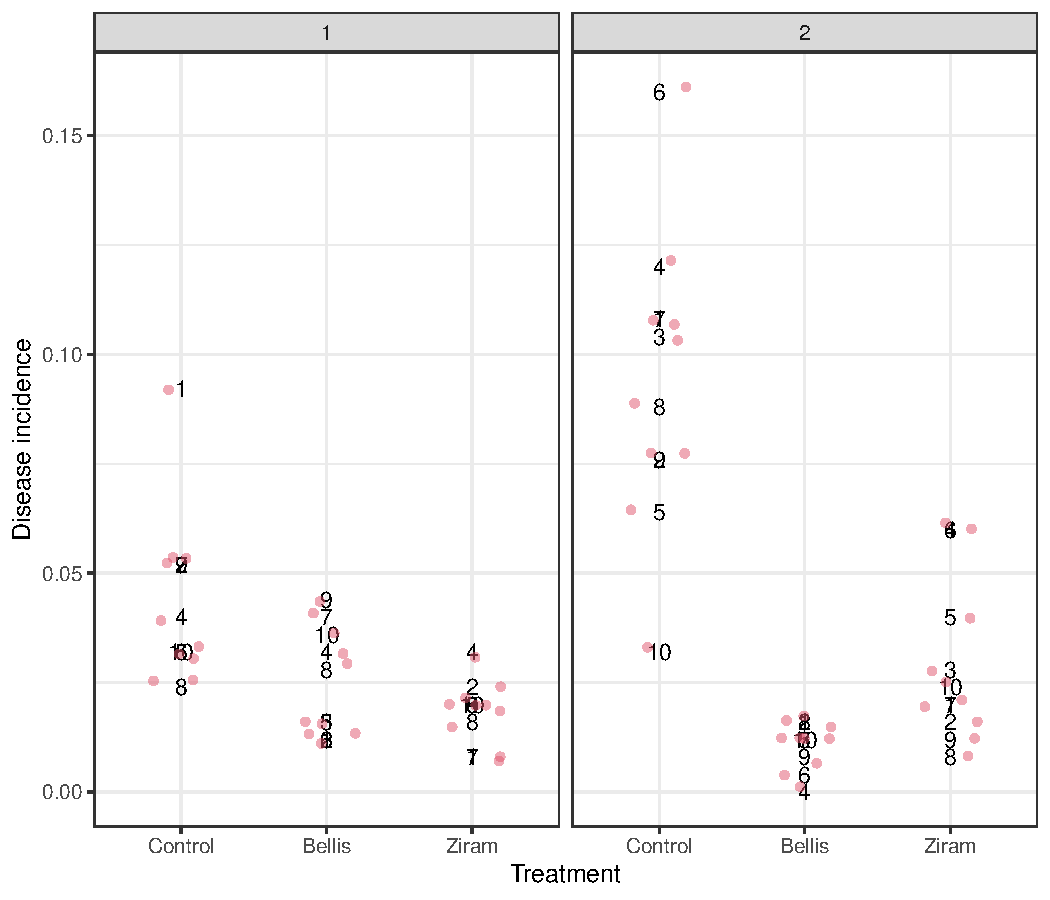
\includegraphics{in_field_files/figure-pdf/unnamed-chunk-4-1.pdf}

}

\end{figure}

\begin{Shaded}
\begin{Highlighting}[]
\NormalTok{mod }\OtherTok{\textless{}{-}} \FunctionTok{glmer}\NormalTok{(diseased}\SpecialCharTok{/}\NormalTok{leaves }\SpecialCharTok{\textasciitilde{}}\NormalTok{ fungicide }\SpecialCharTok{*}\NormalTok{ season }\SpecialCharTok{+}\NormalTok{ (}\DecValTok{1}\SpecialCharTok{|}\NormalTok{tree),}
             \AttributeTok{weights=}\NormalTok{leaves, }\AttributeTok{family=}\NormalTok{binomial, dat)}
\end{Highlighting}
\end{Shaded}

Goodness of fit

\begin{Shaded}
\begin{Highlighting}[]
\FunctionTok{simulateResiduals}\NormalTok{(mod) }\SpecialCharTok{\%\textgreater{}\%} \FunctionTok{testResiduals}\NormalTok{()}
\end{Highlighting}
\end{Shaded}

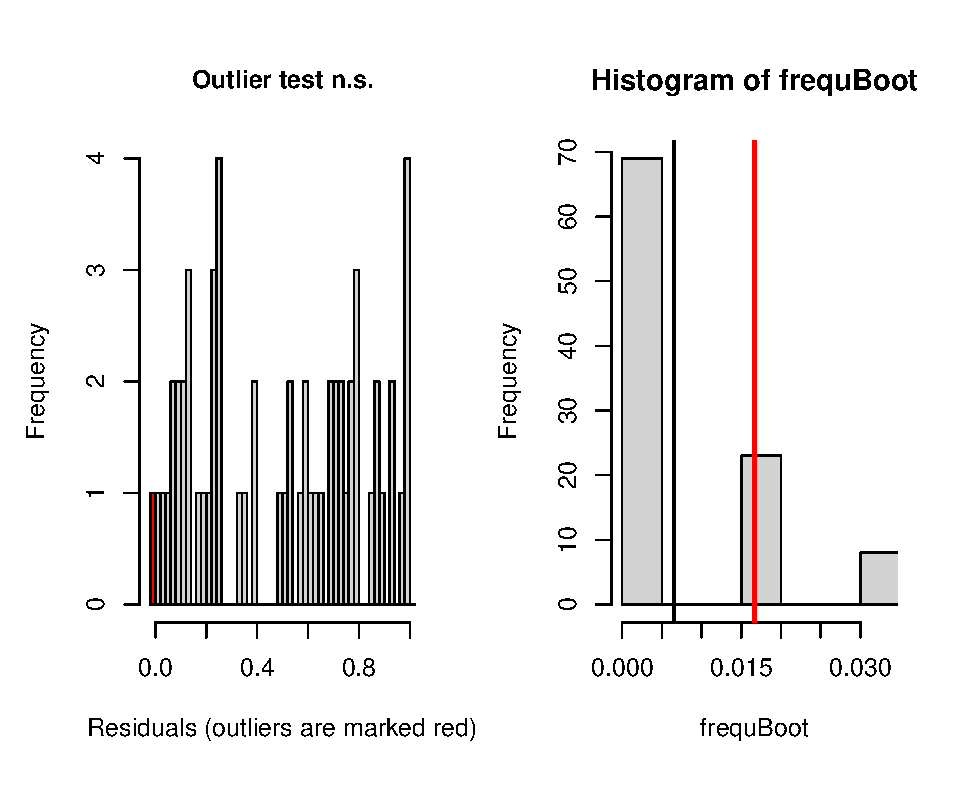
\includegraphics{Residuals plot (in field).eps}

\begin{Shaded}
\begin{Highlighting}[]
\NormalTok{car}\SpecialCharTok{::}\FunctionTok{Anova}\NormalTok{(mod)}
\end{Highlighting}
\end{Shaded}

\begin{verbatim}
Analysis of Deviance Table (Type II Wald chisquare tests)

Response: diseased/leaves
                   Chisq Df            Pr(>Chisq)    
fungicide        160.574  2 < 0.00000000000000022 ***
season            25.222  1        0.000000511051 ***
fungicide:season  41.109  2        0.000000001184 ***
---
Signif. codes:  0 '***' 0.001 '**' 0.01 '*' 0.05 '.' 0.1 ' ' 1
\end{verbatim}

Treatment means comparison

\begin{Shaded}
\begin{Highlighting}[]
\NormalTok{emm }\OtherTok{\textless{}{-}} \FunctionTok{emmeans}\NormalTok{(mod, }\SpecialCharTok{\textasciitilde{}}\NormalTok{ fungicide}\SpecialCharTok{|}\NormalTok{season, }\AttributeTok{type=}\StringTok{"response"}\NormalTok{) }
\NormalTok{res }\OtherTok{\textless{}{-}} \FunctionTok{cld}\NormalTok{(emm, }\AttributeTok{alpha=}\FloatTok{0.05}\NormalTok{, }\AttributeTok{Letters=}\NormalTok{letters,  }\AttributeTok{type=}\StringTok{"response"}\NormalTok{) }\SpecialCharTok{\%\textgreater{}\%} 
   \FunctionTok{mutate}\NormalTok{(}\StringTok{\textasciigrave{}}\AttributeTok{\%Control}\StringTok{\textasciigrave{}}\OtherTok{=}\FunctionTok{abs}\NormalTok{((prob}\SpecialCharTok{/}\NormalTok{dplyr}\SpecialCharTok{::}\FunctionTok{filter}\NormalTok{(.,fungicide}\SpecialCharTok{==}\StringTok{"Control"}\NormalTok{)}\SpecialCharTok{\%\textgreater{}\%} \FunctionTok{pull}\NormalTok{(prob)}\SpecialCharTok{{-}}\DecValTok{1}\NormalTok{)}\SpecialCharTok{*}\DecValTok{100}\NormalTok{)) }\SpecialCharTok{\%\textgreater{}\%} 
\NormalTok{  tibble}

\NormalTok{res }\SpecialCharTok{\%\textgreater{}\%} 
  \FunctionTok{rename}\NormalTok{(}\AttributeTok{Season=}\StringTok{"season"}\NormalTok{) }\SpecialCharTok{\%\textgreater{}\%} 
  \FunctionTok{ggplot}\NormalTok{()}\SpecialCharTok{+}
  \FunctionTok{aes}\NormalTok{(}\AttributeTok{x=}\NormalTok{fungicide, }\AttributeTok{y =}\NormalTok{prob)}\SpecialCharTok{+}
  \FunctionTok{geom\_pointrange}\NormalTok{(}\FunctionTok{aes}\NormalTok{(}\AttributeTok{ymin=}\NormalTok{asymp.LCL , }\AttributeTok{ymax=}\NormalTok{asymp.UCL))}\SpecialCharTok{+}
  \FunctionTok{facet\_wrap}\NormalTok{(}\StringTok{"Season"}\NormalTok{, }\AttributeTok{labeller =}\NormalTok{ label\_both) }\SpecialCharTok{+} \FunctionTok{geom\_text}\NormalTok{(}\FunctionTok{aes}\NormalTok{(}\AttributeTok{label=}\FunctionTok{str\_squish}\NormalTok{(.group)), }\AttributeTok{angle=}\DecValTok{90}\NormalTok{, }\AttributeTok{vjust=}\SpecialCharTok{{-}}\DecValTok{1}\NormalTok{, }\AttributeTok{hjust=}\NormalTok{.}\DecValTok{5}\NormalTok{, ) }\SpecialCharTok{+} 
  \FunctionTok{geom\_jitter}\NormalTok{(}\AttributeTok{data=}\NormalTok{dat}\SpecialCharTok{\%\textgreater{}\%}\FunctionTok{rename}\NormalTok{(}\AttributeTok{Season=}\StringTok{"season"}\NormalTok{) , }\FunctionTok{aes}\NormalTok{(}\AttributeTok{y=}\NormalTok{diseased}\SpecialCharTok{/}\NormalTok{leaves), }\AttributeTok{alpha=}\NormalTok{.}\DecValTok{2}\NormalTok{, }\AttributeTok{width=}\NormalTok{.}\DecValTok{1}\NormalTok{)}
\end{Highlighting}
\end{Shaded}

\begin{figure}[H]

{\centering 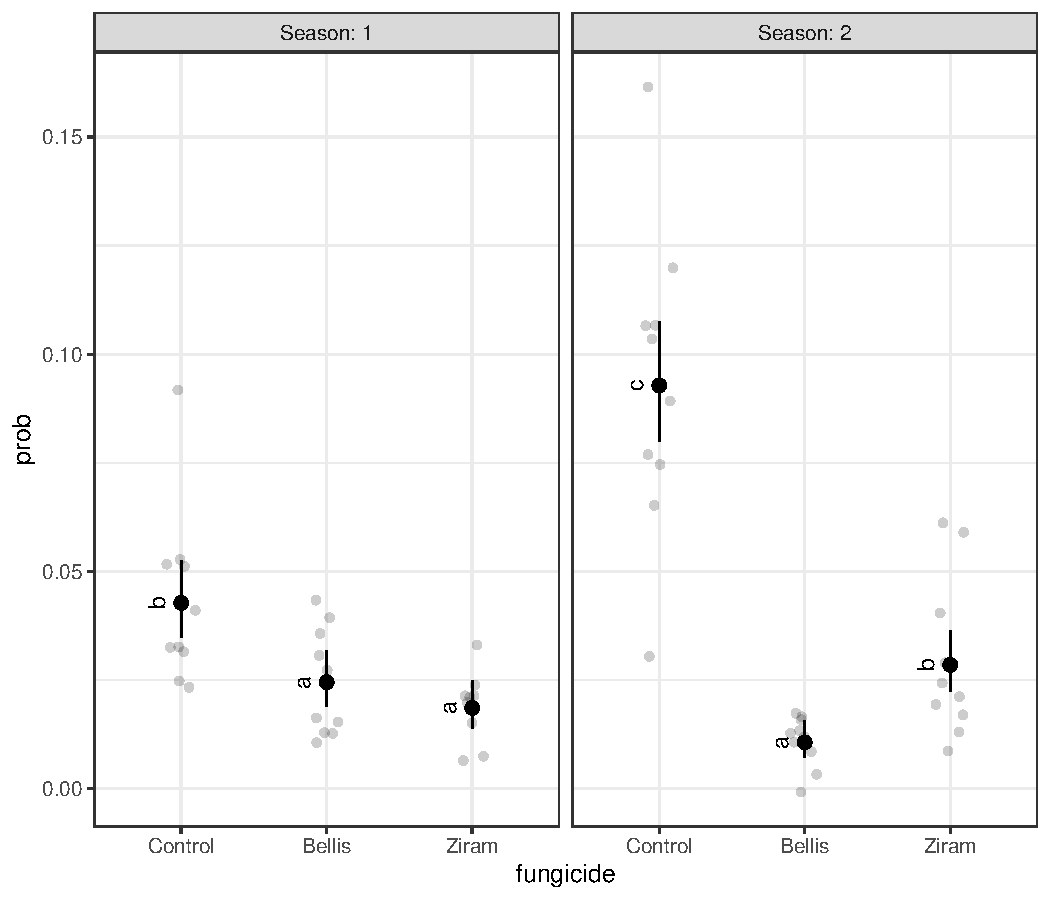
\includegraphics{in_field_files/figure-pdf/unnamed-chunk-8-1.pdf}

}

\end{figure}



\end{document}
